\documentclass[12pt]{article}

\usepackage[margin=1in,top=1in,bottom=1in]{geometry} 
\usepackage{graphicx}              
\usepackage{amsmath, bm}           
\usepackage{amsfonts}              
\usepackage{amsthm}                
\usepackage{hyperref}
\usepackage{natbib}
\usepackage{pdfpages}
\usepackage{booktabs}
\usepackage{multirow}
\usepackage{pgfplotstable}
\usepackage{longtable}
\usepackage{pdflscape}
\usepackage{authblk}
\usepackage{setspace}
\usepackage[title]{appendix}
\usepackage{float}
\usepackage{epigraph,varwidth}

\usepackage{lineno}
\linenumbers

\renewcommand{\epigraphsize}{\small}
\setlength{\epigraphwidth}{0.6\textwidth}
\renewcommand{\textflush}{flushright}
\renewcommand{\sourceflush}{flushright}
% A useful addition
\newcommand{\epitextfont}{\itshape}
\newcommand{\episourcefont}{\scshape}

\makeatletter
\newsavebox{\epi@textbox}
\newsavebox{\epi@sourcebox}
\newlength\epi@finalwidth
\renewcommand{\epigraph}[2]{%
  \vspace{\beforeepigraphskip}
  {\epigraphsize\begin{\epigraphflush}
   \epi@finalwidth=\z@
   \sbox\epi@textbox{%
     \varwidth{\epigraphwidth}
     \begin{\textflush}\epitextfont#1\end{\textflush}
     \endvarwidth
   }%
   \epi@finalwidth=\wd\epi@textbox
   \sbox\epi@sourcebox{%
     \varwidth{\epigraphwidth}
     \begin{\sourceflush}\episourcefont#2\end{\sourceflush}%
     \endvarwidth
   }%
   \ifdim\wd\epi@sourcebox>\epi@finalwidth 
     \epi@finalwidth=\wd\epi@sourcebox
   \fi
   \leavevmode\vbox{
     \hb@xt@\epi@finalwidth{\hfil\box\epi@textbox}
     \vskip1.75ex
     \hrule height \epigraphrule
     \vskip.75ex
     \hb@xt@\epi@finalwidth{\hfil\box\epi@sourcebox}
   }%
   \end{\epigraphflush}
   \vspace{\afterepigraphskip}}}
\makeatother


\newcommand\invisiblesection[1]{%
  \refstepcounter{section}%
  \addcontentsline{toc}{section}{\protect\numberline{\thesection}#1}%
  \sectionmark{#1}}

\doublespacing

\setlength{\LTcapwidth}{8in}

%% \usepackage{caption}
%% \captionsetup{justification=justified}

%% % Setup siunitx:
%% \sisetup{
%%   round-mode          = places, % Rounds numbers
%%   round-precision     = 2, % to 2 places
%% }
%\csname @openrightfalse\endcsname
%\makeatletter\@openrightfalse\makeatother
\newcommand{\kron}{\raisebox{1pt}{\ensuremath{\:\otimes\:}}} 
\newcommand{\lgamma}{\text{lgamma}} 
\newcommand{\digamma}{\text{digamma}} 

\bibliographystyle{ea}
%\bibliographystyle{abbrvnat}

\begin{document}

%\nocite{*}

\title{Quantifying pollen-vegetation relationships to reconstruct ancient forests using 19th-century forest composition and pollen data}

% \author{Andria Dawson\footnote{\url{andria.dawson@gmail.com}}, Department of Statistics, University of California, Berkeley, CA, 94720\\
%   Christopher Paciorek, Department of Statistics, University of California, Berkeley, CA, 94720\\
%   Jason McLachlan, Department of Biological Sciences, 100 Galvin Life Sciences Center, Notre Dame, IN 46556\\ 
%   Simon Goring, Department of Geography, University of Wisconsin-Madison, Madison, WI, 53706\\
%   John W. Williams, Department of Geography, University of Wisconsin-Madison, Madison, WI, 53706\\
%   Stephen Jackson, University of Arizona, Tucson, AZ, 85719}


\author[1, 2]{Andria Dawson}%\footnote{\url{andria.dawson@gmail.com}}}
\affil[1]{Department of Statistics, University of California, Berkeley, CA, 94720}
\affil[2]{Department of Geosciences, The University of Arizona, Tucson, AZ, 85721}
\author[1]{Christopher J. Paciorek}
\author[3]{Jason S. McLachlan}
\affil[3]{Department of Biological Sciences, Notre Dame, IN 46556} 
\author[4]{Simon Goring}
\affil[4]{Department of Geography, University of Wisconsin-Madison, Madison, WI, 53706}
\author[4]{John W. Williams}
%\affil[4]{Department of Geography, University of Wisconsin-Madison, Madison, WI, 53706}
\author[2,5]{Stephen T. Jackson}
\affil[5]{Department of the Interior Southwest Climate Science Center, U.S. Geological Survey, Tucson, AZ, 85721, and Department of Geosciences, University of Arizona, Tucson, AZ, 85721}

\maketitle

\newpage


\begin{abstract}
  Mitigation of climate change and adaptation to its effects relies
  partly on how effectively land-atmosphere interactions can be
  quantified. Quantifying composition of past forest ecosystems can
  help understand processes governing forest dynamics in a changing
  world. Fossil pollen data provide information about past forest
  composition, but rigorous interpretation requires development of
  pollen-vegetation models (PVMs) that account for interspecific
  differences in pollen production and dispersal. Widespread and
  intensified land-use over the 19th and 20th centuries may have
  altered pollen-vegetation relationships. Here we use STEPPS, a
  Bayesian hierarchical spatial PVM, to estimate key process
  parameters and associated uncertainties in the pollen-vegetation
  relationship.  We apply alternate dispersal kernels, and calibrate
  STEPPS using a newly developed Euro-American settlement-era
  calibration data set constructed from Public Land Survey data and
  fossil pollen samples matched to the settlement-era using expert
  elicitation. Models based on the inverse power-law dispersal kernel
  outperformed those based on the Gaussian dispersal kernel,
  indicating that pollen dispersal kernels are fat tailed.  Pine and
  birch have the highest pollen productivities. Pollen productivity
  and dispersal estimates are generally consistent with previous
  understanding from modern data sets, although source area estimates
  are larger. Tests of model predictions demonstrate the ability of
  STEPPS to predict regional compositional patterns.
\end{abstract}

{\bf Keywords:} pollen, fossil, sediment, vegetation, forest, Bayesian,
modelling, expert elicitation, dispersal, calibration, prediction

\newpage
\epigraph{It has been claimed that skilful hunters of old could bring their prey down even if they caught only a fleeting glimpse of its shadow. But still more remarkable appear the performances accomplished to-day by the pollen analyst. Out of pollen from crumbled clay or minute pieces of peat, taken from bits of earthenware or a stone axe, may be constructed a picture of the primeval forests which flourished in the region at the time when the pot or axe dropped, into the bog. This is, however, not the whole story.}{Gunnar Erdtman, 1943}


%\newpage
\section{Introduction}
Understanding changes in past forest composition provides valuable
information about ecosystem response to biotic and abiotic factors at
timescales outside the realm of most direct ecological
observations. Fossil pollen records extracted from sediments of lakes
and mires are a primary source of data about prehistoric forest
composition \citep{brewer2012paleoecoinformatics}. Rigorous estimates
of past forest composition from these records rely on ability to
quantify the relationship between the composition of fossil pollen
assemblages and the composition of the vegetation that produced them.

%% Understanding past forest compositional change provides valuable
%% information about ecosystem response to biotic and abiotic factors
%% at timescales outside the realm of most direct ecological
%% observations.

%% In a rapidly changing climate, there is a need to better quantify
%% climatic processes governing the distributions and dynamics of tree
%% species, and vegetation feedbacks to other components of the earth
%% system. Past forest composition inform about these processes, by
%% allowing us to qunantify ecosystem response to biotic and abiotic
%% factors at timescales outside the realm of most direct ecological
%% observations.


%%  Fossil pollen records extracted from lakes and mires are our primary
%%  source of data about prehistoric forest composition. Rigorous
%%  estimates of past forest composition from these records rely on our
%%  ability to quantify the relationship between the composition of
%%  fossil pollen assemblages and the composition of the vegetation that
%%  produced them.

% Understanding past forest compositional change provides valuable
% information about ecosystem response to biotic and abiotic factors at
% timescales outside the realm of most direct ecological observations
% \citep{jackson2007looking}, particularly with respect to information
% about climatic processes governing the distributions and dynamics of
% tree species \citep{goring2015a, prentice1991vegetation,
%   williams2009rapid, blois2013space, webb1993vegetation} and
% vegetation feedbacks to other components of the earth system
% \citep{matthes2015}. The fossil pollen records extracted from lakes
% and mires are our primary source of data about prehistoric forest
% composition. Rigorous estimates of past forest composition from these
% records rely on our ability to quantify the relationship between the
% composition of fossil pollen assemblages and the composition of the
% vegetation that produced them.

The pollen-vegetation relationship is governed by the processes of
pollen production, transport, and deposition and has been the subject
of empirical and theoretical study for decades \citep{davis1963theory,
  tauber1965, jacobson1981selection, jackson1994pollen,
  jackson1999pollen, sugita2007theory1, sugita2007theory2,
  prentice1988records}. Pollen found in lakes and mires usually
arrives by wind, coming from plants that vary in pollen productivity
and dispersal properties. Some plant taxa are overrepresented in
sedimentary archives while others are underrepresented or absent.
Pollen-vegetation models (PVMs) are designed to make inferences about
past vegetation composition or structure from fossil pollen data.
Some PVMs employ multivariate methods to match pollen assemblages with
vegetation types or biomes; thes include modern-analog based
approaches \citep{overpeck1985quantitative, williams2003variations}
and biomization \citep{prentice1996reconstructing,
  williams1998applying}. Other PVMs relate abundances of individual
plant taxa in vegetation with their abundance in pollen assemblages.
These include pollen/vegetation ratios (R-values)
\citep{curtis1959vegetation, davis1963theory}, linear-regression
\citep{webb1981estimating, bradshaw1985relationships}, extended
R-values \citep{parsons1981statistical, sugita1994pollen,
  sugita2007theory1, sugita2007theory2}, and, most recently, Bayesian
hierarchical models \citep{paciorek2009mapping, garreta2010method}.
In these models, pollen dispersal may be assumed uniform
\citep{davis1963theory, parsons1981statistical}, modeled to decline
away from the source as a simple inverse-square or other function
\citep{webb1981estimating, calcote1995pollen,
  jackson1998quantitative}, or parameterized using various
pollen-transport models, usually based on the Sutton models of
airborne particulate dispersal \citep{prentice1985pollen,
  prentice1988records, jackson1999pollen, sugita2007theory1,
  sugita2007theory2}.

PVMs are ultimately used to reconstruct past vegetation. However, most
models lack the ability to account for uncertainty in a formal,
coherent way. Without some understanding of the uncertainty, it is
difficult to make conclusions about changes across space and/or
time. Our primary goal in this paper is to develop a PVM to estimate
past vegetation composition and its uncertainty. As opposed to working
with individual sites, we treat the data as a cohesive unit, and allow
it to directly inform us about changes in space and time. As in
\citet{paciorek2009mapping}, we use a Bayesian hierarchical spatial
approach (STEPPS) to model pollen counts from a network of ponds as a
function of gridded forest-composition data, taking into account local
pollen dispersal (i.e. pollen sourced from trees within a grid cell
containing a pond) regional pollen dispersal (pollen sourced from
trees in other grid cells), differential pollen production across tree
taxa, and process uncertainty. The statistical model infers production
and dispersal capability by finding parameter values that best
explain the sediment pollen data given known vegetation, within the
structure of how the model represents production and dispersal. The
parameter estimates are collectively informed by all of the pollen and
vegetation data.

PVMs are calibrated using pollen and forest data. Some PVMs, notably
the LOVE/REVEALS family of models \citep{sugita2007theory1,
  sugita2007theory2}, require information about pollen dispersal
properties for individual taxa, which are then used to parameterize
diffusion-based models of particulate transport [e.g.,
  \citet{prentice1985pollen}]. In some cases, PVMs are calibrated
against spatial networks of pollen assemblages extracted from surface-sediment samples that are cross-referenced to contemporary spatial
datasets of vegetation composition and structure
(e.g. \citet{webb1981estimating, williams2003variations}). These
cross-referenced pollen and vegetation datasets are then used to build
empirical models that can be used to infer past forest composition
from fossil pollen assemblages.

Most PVMs are designed to reconstruct vegetation for the relevant
pollen source area of a depositional basin. Previous studies have
shown that the size of the deposition basin may affect the relevant
pollen source area, with sediment pollen from larger lakes providing
better representation of the regional pollen signal
\citep{jacobson1981selection, prentice1985pollen, sugita1994pollen,
  sugita2007theory1}. In the LOVE/REVEALS models
\citep{sugita2007theory1, sugita2007theory2}, background pollen is
estimated based on pollen counts from large lakes, and is then used to
inform local vegetation estimates from pollen counts at smaller
depositional sites. As in LOVE/REVEALS, STEPPS also divides pollen
dispersal into local and non-local components, however, only
LOVE/REVEALS requires estimates of productivity, pollen-deposition
velocity, and atmospheric conditions, as model inputs. It is important
to note that the operational definition of local varies among models,
and within the literature. In \citet{jacobson1981selection}, local is
defined as being within $10^2$ m of the depositional basin; in our
case, local refers to the grid cell containing this basin, which is
$10^3$ m - an order of magnitude larger.

Most spatially calibrated PVMs are not explicitly process-based,
although sometimes the parameters in these empirical models give
insight into process (e.g. the y-intercept in linear regression models
provides an estimate of pollen dispersed from outside the
vegetation-sampling area \citep{webb1981estimating}).  In contrast,
Bayesian hierarchical models can be spatially calibrated and designed
to include parameters that represent processes in pollen production,
transport, and deposition \citep{paciorek2009mapping}. While both
STEPPS and LOVE/REVEALS account for production and dispersal, neither
model is fully mechanistic (e.g., explicitly based on
particle-dispersal dynamics). The strength of the Bayesian PVM
presented here relative to LOVE/REVEALS and other PVMs is its ability
to estimate vegetation, process parameters, and uncertainty, by
accounting for spatial dependence and borrowing information across
space. Parameter estimates are used to estimate spatial maps of
vegetation, and their uncertainty, even at locations without extant
pollen data. In addition, we avoid the need for \textit{a priori}
parameter estimates (e.g. of pollen productivity, atmospheric
conditions, or settling velocity) using a coherent hierarchical
framework. Requiring parameter estimates is not an impediment
\textit{per se}, but some of the inputs required for other PVMs may be
difficult to measure or quantify, or variable through time and/or
space \citep{jackson1994pollen, jackson1999pollen}.

Unlike many other PVMs, STEPPS assumes that depositional basin size
does not affect the distance weighting of the surrounding
vegetation. This is in part a consequence of the spatial resolution of
the 8 km gridded vegetation data sets used here; our ability to
resolve fine-scale compositional patterns near depositional basins is
restricted by the coarseness of the available vegetation
data. However, all deposition sites regardless of size receive much of
their pollen from regional sources and hence are sensitive to
broader-scale vegetation patterns and gradients
\citep{bradshaw1985relationships, prentice1987quantitative,
  jackson1991pollen, sugita2007theory1, sugita2007theory2}. Although
the lack of higher-resolution vegetation-sampling likely imposes some
error \citep{bradshaw1985relationships, prentice1987quantitative,
  jackson1990}, our goal is to predict vegetation at a regional scale
and as such we do not expect to resolve fine-scale local
heterogeneities.


%% The main advantage of this approach is the ability to borrow
%% information across space to estimate governing parameters and their
%% uncertainty at a regional scale, without the reliance on prior
%% quantification of ecological or physical processes.


%% Bayesian hierarchical models,
%% however, are flexible and can be designed to include parameters that
%% represent processes in pollen production, transport, and deposition
%% \citep{paciorek2009mapping}.

Extending PVMs to make inferences about palynological processes and
vegetation composition for times other than the time of calibration
requires the assumption that pollen-vegetation relationships are
constant. This assumption of constancy seems reasonable at first
approximation; although tree taxa may vary in their productivity and
dispersal both in space and time, the relative differences among taxa
should be less variable \citep{parsons1981statistical}.  The magnitude
of both compositional and structural modification of vegetation by
human land-use in the past four centuries in eastern North America and
elsewhere, this assumption merits investigation and testing
\citep{kujawa2016}. Recent human land use has significantly altered
forest composition and structure. Most contemporary forests differ in
density, biomass, size structure, and age structure from
pre-settlement forests \citep{leahy2003comparison,
  schulte2007homogenization, rhemtulla2009legacies, goring_witness},
and ecotonal gradients in forests in the upper Midwestern US were
steeper in pre-settlement forests than they are now
\citep{goring_witness}. Land clearance, forest management practices,
and successional processes have led to fundamental changes in forest
composition, and hence early-successional trees such as poplar and
some maple species are more abundant now than in the 19th century
\citep{thompson2013four, goring_witness}. The overall pattern of
forest mosaics in the region has also changed - at broad scales
forests are more spatially homogeneous (e.g., forest management
practices and recovery from land clearance) while at finer scales
forests are more heterogeneous (e.g., locally idiosyncratic
disturbance or land-use legacies) \citep{thompson2013four,
  wang2007spatial, li2015drivers, goring_witness}. Finally, fire
suppression during the 20th century may have led to increasing forest
density and changes in abundance of fire-adapted species
\citep{nowacki2008demise}. Critically however, the nature of change
across the region varies; for example, fire suppression has led to
higher biomass in northern Minnesota, while clearance and regeneration
has resulted in lower biomass in southern Wisconsin and Michigan
\citep{goring_witness}.

These changes in forest composition, structure, and landscape pattern
may have directly influenced pollen production and dispersal
\citep{kujawa2016}.  Pollen production, for example, may be greater
for trees growing in the open or at forest edges
\citep{feldman1999cost}.  Pollen dispersal is affected by properties
of both the forest canopy and the land surface
\citep{jackson1999pollen}.  A more serious issue for pollen-vegetation
relationships may be that at the landscape level, many contemporary
forests have no historical analogues \citep{goring_witness}. Shifting
forest composition can alter pollen-vegetation relationships because
of the Fagerlind effect, in which relative pollen representation of
one taxon is affected by that of all other taxa contributing to an
assemblage \citep{prentice1988records}. It is possible to account and
correct for the Fagerlind effect using ERV models \citep{prentice1986,
  jackson1995exploration}, but empirical corrections are contingent on
particular vegetational contexts \citep{jackson1998quantitative}.

Most PVMs are calibrated using contemporary forest data; few studies
have examined settlement-era pollen-vegetation relationships
\citep{schwartz1989predicting}. Although some have used historical
forest cover maps to validate models based on modern relationships
\citep{nielsen2004modelling}, a recent study has shown that
pollen-based paleoclimate reconstructions calibrated with
settlement-era pollen data differ significantly from those using
modern pollen data \citep{st2014bias} suggesting that shifts in
pollen-climate relationships have occurred across the region. The
compilation of settlement-era Public Land Survey (PLS) forest
composition records from the western Great Lakes region
\citep{bourdo1956review, schulte2001original,
  almendinger1996minnesota, liu2011broadscale, goring_witness}, along
with a new dataset of settlement-era fossil pollen records from the
upper Midwest \citep{kujawa2016}, largely drawn from the Neotoma
Paleoecological Database (www.neotomadb.org), provides an opportunity
to calibrate a PVM for the early to mid-19th century, thus avoiding
the effects of settlement, agriculture, and industrialization.

Cross-referencing settlement-era forest composition with appropriate
fossil data requires identification of pollen samples that are
contemporaneous with the settlement era.  In eastern North America,
land clearances during Euro-American settlement led to increases in
certain agricultural and weedy plant taxa; these increases can be used
as direct biostratigraphic markers of settlement in pollen records. Of
these, the rise in ragweed (\textit{Ambrosia}) abundance is generally
the most prominent \citep{mcandrews1988human} and is widely used by
palynologists to identify the Euro-American settlement horizon
(defined as the sample immediately preceding increases in indicator
taxa). Identifying the settlement horizon in this way requires
interpretation of pollen sequences; the uncertainty associated with
this interpretation has not been assessed to date. Here we use expert
opinion from four paleoecologists to reduce bias and quantify
uncertainty associated with the identification of biostratigraphic
signals. Results from this exercise are used to construct a
settlement-era pollen-calibration data set.

Towards our goal of predicting vegetation and uncertainty, we develop
and calibrate a Bayesian hierarchical PVM based on the STEPPS
(Spatio-Temporal Empirical Prediction from Pollen in Sediments) model
\citep{paciorek2009mapping}. We calibrate the PVM using the
settlement-era PLS forest composition and pollen datasets, and use
these calibration results to predict settlement-era vegetation
composition for the upper Midwestern US. We assess our ability to
predict vegetation composition by comparing these spatial predictions
with the PLS data. With both prediction and understanding in mind, we
test variations of the calibration model against the data and compare
results to our current scientific understanding of pollen
processes. Specifically, we test and compare two standard isotropic
pollen-dispersal kernels. We apply the PVM results to develop new
estimates of relative pollen productivity and source area, and assess
the relative importance of local and non-local pollen sources.

% In this work, our primary goal is to develop a PVM to estimate past
% vegetation composition and its uncertainty. There are several
% quantitative methods that have been used to develop vegetation
% reconstructions, however these models lack the ability to account for
% uncertainty in a coherent way. Without understanding of the
% uncertainty, it is impossible to make definitive conclusions about
% changes across space and/or time. Here we let the data directly inform
% us about changes in space and time, and their uncertainty. To achieve
% this goal of reconstructing vegetation, we aim to develop a
% statistical model that accounts for and quantifies the processes of
% pollen production and dispersal. The success of the PVM is measured by
% its ability to predict the vegetation data and estimate production and
% dispersal parameters that agree in general with our scientific
% understanding of pollen processes. A secondary goal is to use the PVM
% to improve our understanding of the underlying processes, which we do
% by testing variations of the calibration model against the data.

\section{Data and Methods}

\subsection{Data}

\subsubsection{Spatial domain}

The study area is the upper midwestern US (UMW), including Minnesota,
Wisconsin, and Michigan (see Fig.~\ref{fig:pie}).  This region
includes two major ecotones: the ``Tension Zone'' between northern
mixed forests and temperate broadleaved deciduous forests
\citet{curtis1959vegetation}, and the prairie/forest/savanna ecotone.
Both of these ecotones have been heavily modified by contemporary land
use \citep{goring_witness}. We focus on the UMW because of the strong
vegetation gradients associated with these ecotones and because of the
dual availability of an integrated network of pre-settlement
forest-composition estimates \citep{goring_witness} and high density
of pollen sequences spanning the settlement era.

\subsubsection{Public Land Survey (PLS) data}
Prior to major European settlement, the US General Land Office
conducted a Public Land Survey (PLS) throughout much of the United
States to simplify the sale of federal lands. The PLS mapped the
United States west and south of Ohio on a 1$\times$1 mile grid for the
sale of public lands \citep{stewart1935public,
  white1983history}. Surveyors marked section corners with stakes, and
recorded the closest two to four trees, measuring the distance from
tree to point center, azimuth, tree diameter and the (often
idiosyncratic) common name of these trees
\citep{mladenoff2002narrowing}.

Data from the PLS constitutes a systematic survey of the forest before
settlement, and has been used by foresters, ecologists, and historians
to learn about ecosystem and land-use change. In the UMW, the survey
was conducted between 1834 and 1907 \citep{stewart1935public}.

Recently these point-level data have been aggregated across the UMW to
a 64 km$^2$ grid (8$\times$8 km) on an equal-area Albers projection
(proj4: +\textit{init}=\textit{epsg}:3175) and standardized to account
for changing survey instructions through time (cf. Stewart, 1935) and
to provide sufficient spatial resolution for regional-scale analysis
\citep{goring_witness}.  This aggregation results in an average count
of 134 trees per grid cell. This tree count per cell is low, but
ecological patterns and regional structure of the dominant forest taxa
are evident because of the uniforma spatial sampling
\citep{goring_witness}. In a given grid cell, the raw data provide
noisy estimates of composition proportions because of the limited
number of trees per cell. Instead, we use composition estimates
provided by \citet{paciorek2015}, who applied a statistical model that
borrows information across nearby grid cells to estimate the
composition proportions in each grid cell with uncertainty. Here we
work with these PLS composition estimates. These estimates are not
data in the true sense, but assumed to be fixed for our purposes and
are hereafter referred to as PLS data.

\subsubsection{Tree taxa}

For the UMW domain, \citet{goring_witness} report fifteen tree taxa,
although the full dataset contains 28 taxa.  Most taxa are resolved to
the level of genera, and the list of taxa includes ``No Tree'' (21\%
of points) when surveyors did not find a tree within a reasonable
distance, ``Unknown Tree'' (0.001\% of points) when the common name
used to identify the tree could not be resolved, and ``Other
Hardwood'' (0.02\% of points) when the surveyed tree was clearly a
hardwood, but could not be resolved beyond that level. We focus on a
subset representing two functional groups (Deciduous and Coniferous
taxa) composed of 10 tree genera that include the most abundant taxa
as well as less-abundant but ecologically significant taxa. These taxa
are: ash, beech, birch, elm, hemlock, maple, oak, pine, spruce, and
tamarack (see Table~\ref{table:pollen_acc} for scientific name
translations). The remaining tree taxa, including ``Unknown Tree'',
are aggregated to ``Other Hardwood'' or ``Other Conifer'', which
amount to 10\% and 7\% of the included trees respectively.``No Tree''
is excluded from further analysis.

% \textit{Abies}, \textit{Acer}, \textit{Betula},
% \textit{Fagus}, \textit{Fraxinus}, \textit{Larix}, \textit{Picea},
% \textit{Pinus}, \textit{Quercus}, \textit{Tsuga}, \textit{Ulmus}

% The separation of other
% hardwood and conifers allows the calibration model to treat ecological
% group separately, teasing out inherent differences between conifer and
% deciduous pollen production, although variability in production and
% dispersal within each group is large.

\subsubsection{Pollen data}

Advances in paleoecoinformatics \citep{brewer2012paleoecoinformatics,
  grimm2013encyclopedia} have made it possible to easily access and
query large datasets using tools such as the multi-proxy
Pliocene-Quaternary database Neotoma (\url{neotomadb.org}). The
development of the Neotoma API (\url{api.neotomadb.org}) has provided
a foundation for the development of a map-based search interface - the
Neotoma Explorer (\url{apps.neotomadb.org/explorer}) - and the neotoma
package for R \citep{goring2015}. Using these tools we identified 176
sedimentary pollen records in the Neotoma database from the UMW. To be
considered for settlement-era calibration, records must contain a
sample deemed representative of settlement-era vegetation; for this
reason, we considered only records that included multiple pollen
samples from the last 2000 years (under the assumption that one of
these samples can be deemed representative). An additional 57 records,
not available from Neotoma at the time of this project, were
contributed by independent researchers \citep{kujawa2016}. These
additional records include 9 pollen-count time-series records and 48
records that consist only of the core-top and pre-settlement
assemblages, hereafter referred to as before-after records. The dating
controls available for the identified pollen records varied. To form
our calibration data set we primarily relied on biostratigraphic
markers of EuroAmerican land clearance.  As a result radiometric and
other dating controls were not explicitly considered during the pollen
record screening process (but will be considered in the formation of
the prediction data set). The new settlement-era pollen dataset is
described in \citet{kujawa2016}.

Pollen records are obtained from morphological assignment of
individual pollen grains from sediment samples into groups that
correspond with plant taxa, which is a labor-intensive and
skill-dependent process. Each pollen count represents a sample from a
larger population \citep{maher2012assessment, maher1981statistics},
although uncertainty from pollen identification and counting is
negligible for regional-to-global-scale syntheses focused on the most
common taxa from lake and mire sediments \citep{webb1978sensing,
  webb1978mapped}. These data are collected by independent researchers
and as such require the standardization of pollen taxonomies to
account for differing nomenclature and taxonomic resolution. Here
pollen taxonomies were standardized using the STEPPS translation table
from \url{neotoma}, which is reported as supplemental material.

\subsubsection{Elicitation of evidence for settlement in pollen
  records}

Widespread land clearance during Euro-America settlement provided
habitat for many ruderal plants, resulting in increases in
non-arboreal taxa that are evident in pollen records
\citep{mcandrews1988human}. In the UMW, significant
increases in ragweed (\textit{Ambrosia}), docks and sorrels
(\textit{Rumex}), and grasses (\textit{Poaceae}) typically mark this
settlement horizon.

Here we use expert elicitation to identify the representative
settlement horizon sample, defined to be the sample preceding the
increase in agricultural indicator species, at each of the 185 sites
with pollen count time series data. All expert elicitation relies on
judgment, and there is often significant variability in expert's
determination of true signals \citep{bond2007you, bond2012makes}. The
degree of uncertainty resulting from expert identification of
``settlement'' likely varies among sites as a result of the temporal
density of pollen samples, time-averaging of sediments, the rapidity
of forest clearance and landscape transformation, the pollen
representation of dominant trees, which can dampen or amplify the
ragweed signal, and expert knowledge of the region and the
late-Holocene history of the site. At some sites, the settlement
horizon is unambiguous, while at others the transition is less clear
(see App.~\ref{append}, Fig.~\ref{fig:elicit}).

In the interest of reducing bias and quantifying uncertainty, we: 1)
use consistent methodology to identify the settlement horizon in the
pollen records, and 2) assess the variability in settlement horizon
assignment among analysts. Four expert palynologists (Goring, Jackson,
St. Jacques, Williams) participated in the elicitation exercise. Each
expert was provided with pollen diagrams depicting proportional
changes through time as a function of depth for the ten most abundant
arboreal plus key indicator taxa for the last 2000 years as determined
by the default Neotoma age-depth models. Experts were prohibited from
relying on stratigraphic dates (radiocarbon or other) or age-depth
model estimates of sample age. Experts were instructed to report the
horizon as non-identifiable when they could not distinguish the
settlement horizon, and to note the uncertainty of their settlement
horizon assignments, with or without justification. Expert
identifications were subsequently checked against age assignments
based on age-depth models either obtained from Neotoma or constructed
using original age controls and the Bacon age model
\citep{blaauw2011flexible}.  Results from this exercise were used to
define depths associated with settlement horizon samples and their
uncertainty. Pollen samples corresponding to the selected settlement
horizon depths were included in our calibration data set. Expert
elicitation results are included as supplementary material.

% To calibrate a PVM against PLS forest composition data, prior to major
% anthropogenic disturbance, requires pollen data that is
% contemporaneous with the pre-settlement era. Pollen assemblages from
% past times are obtained by coring depositional environments including
% lakes, mires, and forest hollows, among other locations, in which the
% cell walls of deposited pollen are preserved. Contemporaneous pollen
% assemblages are identified largely using the estimated age of the
% pollen sample, obtained from chronologies constructed using classical
% \citep{blaauw2010methods} or Bayesian \citep{blaauw2011flexible,
%   buck1999bcal, blaauw2005radiocarbon, ramsey1995radiocarbon}
% methods. Chronologies are developed using dated stratigraphic control
% points from within a core, which may be geochronological (dated
% material), geostratigraphic (e.g., the ``modern'' core top), and
% sometimes biostratigraphic (changes in pollen assemblages associated
% with dated changes on the landscape). Geochronological control points
% are dated using radiometric dating (typically radiocarbon
% (${}^{14}C$), but sometimes lead-210 ($^{210}$Pb) or cesium-137
% ($^{137}$Cs)), although these dates are uncertain due to analytical
% errors during the laboratory radiometric dating process
% \citep{ward1978procedures}, the conversion of radiocarbon to calendar
% years \citep{reimer2013intcal13}, and potential differences between
% age of macrofossil material and age of sediment
% \citep{blois2011methodological}. Geostratigrahic markers may have
% fewer sources of uncertainty - the core top age is assumed to be the
% year of sampling, although sedimentary mixing of the upper sediment
% during sampling does introduce some uncertainty. Finally,
% biostratigraphic control points are determined by examination (usually
% visual) of changes in pollen assemblages throughout a core, and are
% typically only used when there a well established understanding of a
% large-scale event that led to consistent changes in the pollen
% records.

% The pollen sample that best represents pre-settlement times can be
% identified using the pollen sample age, as estimated by an age-depth
% chronology. However, age-depth modelling of sediment requires
% assumptions about depositional processes that can be difficult to
% quantify, resulting in potentially uncertain age-depth
% predictions. Instead, we rely on a panel of experts to identify a
% biostratigraphic change in pollen records associated with European
% settlement, thus reducing bias associated with biostratigraphic marker
% identification, and eliminating the need to assign a date to a
% representative pollen sample.

% Widespread land clearance during European settlement provided habitat
% for many ruderal plants, resulting in increases in non-arboreal taxa
% in pollen time series \citep{mcandrews1988human}. In the Upper
% Midwest, significant increases in ragweed (\textit{Ambrosia}), docks
% and sorrels (\textit{Rumex}), and grasses (\textit{Poaceae}) typically
% mark this settlement horizon. Here we use expert elicitation to
% identify the representative pre-settlement sample - the sample that
% falls immediately before these increases in agricultural indicator
% species. All expert elicitation relies on judgement. The uncertainty
% in pre-settlement sample identification varies widely among sites as a
% result of the chronological density of pollen samples
% \citep{liu2012temporal}, time-averaging of sediments, the rapidity of
% forest clearance and landscape transformation, and the pollen
% representation of dominant trees, which can dampen or amplify the
% \textit{Ambrosia} signal. At some sites, the settlement horizon is
% unambiguous, while at others the transition is less clear (see
% Fig.~\ref{fig:elicit}).

% For this study, in the interest of reducing uncertainty, we want to:
% 1) identify pre-settlement samples using consistent methodology, and
% 2) assess the variability in assignment of pre-settlement among
% analysts. To address these questions, we asked a team of four expert
% palynologists to identify the pre-settlement sample for 185 pollen
% records. Experts were provided with pollen diagrams depicting
% proportional changes through time as a function of depth for key
% indicator species and the ten most abundant arboreal taxa. Experts
% were prohibited from relying on stratigraphic dates (radiocarbon or
% other) or age-depth model estimates of sample age. In the case that
% there was no distinguishable pre-settlement sample, experts were
% instructed to report NA. In the case that experts were uncertain about
% their pre-settlement sample assignment, they were instructed to note
% this, with or without justification. Results from this exercise are
% used to define depths associated with pre-settlement samples. Pollen
% samples associated with these depths are placed into our calibration
% data set.


\subsection{Models}
\label{sec:models}

In this section we describe the PVM. In our workflow,
vegetation reconstruction is composed of two phases: calibration and
prediction. In section~\ref{sec:cal}, we describe the calibration
model used to estimate the parameters that describe the processes that
link vegetation composition to sediment pollen through pollen
production and dispersal. Then, in section~\ref{sec:pred}, we describe
the prediction model used to estimate settlement-era vegetation
composition. In section~\ref{sec:imp} we describe computational
software and tools used to fit the models.

%  the methodological foundation for rigorous
% reconstruction of past forest composition from fossil pollen data and
% all scripts are made publicly available at GitHub (link).

\subsubsection{Calibration model}
\label{sec:cal}

Here we describe the calibration model used in the first phase of
vegetation reconstruction. We first provide an overview of the model
and then introduce the mathematical notation.

The observed pollen counts are a function of the vegetation on the
landscape; i.e., the composition and abundance of trees on the
landscape determines (in part) the composition and abundance of pollen
deposited in the sediment. How much pollen the surrounding vegetation
contributes is a complex function of forest characteristics (e.g.,
composition, structure, patchiness, spatial stationarity), climate
(including wind), pollen productivity, grain size and morphology,
topography, and proximity of the vegetation to a deposition basin.

We work on an 8 km grid defined by the resolution of the gridded PLS
data and define each deposition site as having both local and
non-local pollen contributions. Local contributions are made by the
vegetation within the same grid cell as a site, and non-local
contributions are made by vegetation from other grid cells. The
relative contribution of local versus non-local pollen is determined
by a model parameter, with the restriction that the sum of all
contributions from the pollen source area must be one. We emphasize
that here ``local'' refers to pollen from an area much larger than
what would usually be referred to as such.

Contributions from non-local grid cells are not all equal; their
relative contributions are distance-weighted according to a dispersal
kernel, which determines how likely it is for pollen to travel from
one grid cell to another. Dispersal is a well-studied phenomenon, and
there is no consensus on a single best dispersal kernel; dispersal
kernels vary in function complexity and flexibility, and some are
better suited in certain cases than others
\citep{clobert2012dispersal}. Given this, we test two dispersal
kernels, both of which have been used to model pollen dispersal
\citep{clobert2012dispersal}. The considered dispersal kernels are
isotropic, meaning they depend only on the distance of the tree to the
deposition site and not on the absolute position or direction. In
reality, dispersal may not be isotropic, owing to prevailing wind
directions during pollen-dispersal seasons, regional topography,
surface roughness, and vegetation patchiness on the
landscape. However, isotropic dispersal kernels are a reasonable and
widely used approximation \citep{sugita2007theory1,
  sugita2007theory2}, because turbulent atmospheric mixing below the
boundary layer tends to smooth out anisotropies. We define a maximum
dispersal distance that determines an upper limit to the distance that
pollen is able to disperse from the source; this reduces computation
without a significant loss of information.

Here, we choose two kernels that are representative of the short- and
long-tail kernel classes, the Gaussian kernel (GK) and the inverse
power-law kernel (PLK), and compare between these generalized
functional forms. The GK is often used as a reference against more
leptokurtic kernels such as the PLK and can represent dispersal
through diffusion. While the GK has a simpler mathematical
representation, fatter-tailed kernels (such as the PLK) in general
perform better than those with thinner tails (like the GK or
Exponential) when modelling pollen dispersal
\citep{devaux2007modelling, austerlitz2004using}. However, pollen
dispersal data needed to validate pollen dispersal models are
generally unavailable, especially at the large spatial scales required
to adequately test long-tailed kernels \citep{clobert2012dispersal}.

To determine how much pollen a grid cell contributes to a deposition
site such as a pond, the vegetation composition proportion vector is
first scaled by taxon-specific parameters that account for
differential pollen production among tree species. The local
contribution is determined by the scaled vegetation vector for the
grid cell that contains the pond. For all grids cells in the domain
that do not contain the pond, their scaled vegetation vectors are
multiplied by the respective weights assigned by the dispersal kernel
(which depend on the distance to the pond and the kernel
parameters). The total non-local contribution is the sum of the scaled
and weighted vegetation vectors over all grid cells that do not
contain the pond. The relative importance of the local and non-local
contributions is determined by the local strength parameter, and the
sum of the local and non-local contributions determines the predicted
sediment pollen at the pond.

\subsubsection*{Calibration model details}

Here we give a mathematical description of the calibration model. As
described, the spatial domain is regular grid composed of 64 km$^2$
discrete cells, but the underlying vegetation composition and
dispersal spatial processes are continuous functions of space. Spatial
cells are indexed by $s=1,\ldots,S$, and for the full UMW
spatial domain $S=8013$. All grid cells in the domain are potential
sources of pollen.

Pollen produced by vegetation within each grid cell can be deposited
within that grid cell or dispersed into the neighborhood around that
grid cell. For grid cell $s_i$, the pollen produced by taxon $p$
within that cell that remains local is given by
\begin{linenomath*}
\begin{equation}
\gamma \phi_p r_p(s_i),
\end{equation} 
\end{linenomath*}
where $\gamma$ is the proportion of pollen produced in $s_i$ that is
deposited in $s_i$, $\phi_p$ is the scaling factor that accounts for
differential production, and $r_p(s_i)$ is the proportional abundance
of vegetation of taxon $p$ in $s_i$.

The remaining $1-\gamma$ proportion of pollen produced in $s_i$ is
dispersed to other grid cells according to an isotropic dispersal
kernel centered at $s_i$. The dispersal kernel weights all pollen
dispersing away from the focal cell as a function of the distance from
$s_i$ to any neighboring cell $s_k$ by $w(s_i, s_k)$.

The two dispersal kernels considered are the GK, defined as
\begin{linenomath*}
\begin{equation}
  w_g(s_i, s_k) = \exp\left( - \frac{d(s_i, s_k)^2}{\psi^2} \right),
\end{equation}
\end{linenomath*}
where $d(s_i,s_k)$ defines the distance between cells $s_i$ and $s_k$
and $\psi>0$ is a parameter that describes the spread of the
kernel, and the PLK, defined as
\begin{linenomath*}
\begin{equation}
w_{pl}(s_i, s_k) = \frac{(b-2)(b-1)}{2 \pi a^2} \left( 1 + \frac{d(s_i, s_k)}{a} \right)^{-b},
\end{equation}
\end{linenomath*}
where $a>0$ and $b>2$ are parameters that determine the kernel
shape. As expected, the weight assigned by both kernels is a
decreasing function of distance - less pollen is distributed farther
away.
 
Pollen produced by taxon $p$ dispersing from $s_i$ to $s_k$ is then
calculated as
\begin{linenomath*}
\begin{equation}
(1-\gamma) \phi_p r_p(s_i) w(s_i, s_k),
\end{equation}
\end{linenomath*}
where $w \in \{w_{g}, w_{pl} \}$.

So far we have characterized the model from a source-based
perspective, describing how pollen disperses from the grid cell in
which it was produced. To quantify vegetation we need to interpret the
counts of pollen grains from the sedimentary record from site $i$ in
grid cell $s_{i}$. These pollen grains were produced in and dispersed
from grid cells within the maximum dispersal distance, and have been
deposited, preserved, and counted. The pollen arriving at site $i$ is
equal to the sum of the locally deposited pollen plus the pollen
dispersed to $s_i$ from other grid cells in the domain that are within
the maximum dispersal distance of $s_i$. Therefore the pollen of taxon
$p$ arriving at pond $i$, referred to as $r_{i,p}^{\text{pol}}$, is
given by
\begin{linenomath*}
\begin{equation}
r_{i,p}^{\text{pol}} = \gamma \phi_p r_p\bigl(s_i\bigr) + \frac{1}{\Omega} (1-\gamma) \phi_p \sum_{s_k \neq s_i } r_p(s_k) w\bigl(s_i, s_k\bigr)
\label{eq:arriving}
\end{equation}
\end{linenomath*}
where $\Omega$ is a normalizing constant equal to the sum of the
weights of all the cells to which pollen can be dispersed, defined to
be a circle of radius 700 km. Note that $\Omega$ depends on the
dispersal kernel, and therefore varies as a function of dispersal
kernel parameters. However, for a given a set of parameter estimates,
$\Omega$ is constant across the domain.

Finally, we need to relate the arriving pollen $r_{i,p}^{\text{pol}}$
quantified in Equation~\ref{eq:arriving} to the pollen count data. To
do this, we consider that the pollen data are overdispersed - the
counts are more variable than we might expect if they were
multinomially distributed. This overdispersion is at least in part
(and perhaps mostly) attributed to heterogeneity in the pollen
production and dispersal processes that is not accounted for in our
mathematical characterization but is also an artifact of the
comparison of pollen counts at a point location (the depositional
site) situated anywhere within a focal grid cell to a grid-based
estimate of pollen deposition. Therefore, we model the pollen counts
at depositional site $i$, denoted by $\bm{y}_i=(y_{i1}, \ldots,
y_{iP})$, with a Dirichlet-multinomial (DM) distribution, a compound
distribution used to account for overdispersion in multinomial count
data (that simplifies to the multinomial distribution in the case of
no overdispersion). We have that
\begin{linenomath*}
\begin{equation}
\bm{y}_i \sim DM (n_i, \bm{r}_i^{\text{pol}}),
\label{eq:DM}
\end{equation}
\end{linenomath*}
where $\bm{r}_i^{\text{pol}} = (r_{i,1}^{\text{pol}}, \ldots,
r_{i,P}^{\text{pol}})$ and $n_i$ is the number of pollen grains
counted at site $i$.  The precision $\alpha_i$ of the distribution is
equal to the sum of Equation~\ref{eq:arriving} over all taxa
\begin{linenomath*}
\begin{equation}
\alpha_i = \sum_{p=1}^P \Bigl[\gamma \phi_p r_p\bigl(s_i\bigr) + \frac{1}{\Omega} (1-\gamma) \phi_p \sum_{s_k \neq s_i } r_p(s_k) w\bigl(s_i, s_k\bigr)\Bigr].
\label{eq:alpha}
\end{equation}
\end{linenomath*}
Note that the precision is affected by the proximity of a depositional
site to the domain boundary. We do not have PLS data outside of the
defined UMW domain, so we cannot quantify the pollen dispersed from
vegetation outside the domain arriving at depositional sites in our
domain. The repercussion of this is that the sum of weights of the
grid cells contributing pollen to sites close to the domain boundary
is less than the sum of weights of the total potential contributing
neighborhood, defined as $\Omega$. The result of having a smaller
contributing neighborhood is that the local pollen contribution is
effectively up-weighted relative to the non-local contribution.This
edge effect will have the greatest impact at sites that are close to
the boundary and near regions of vegetation that contribute pollen
which are not accounted for (some sites are near the boundary but are
surrounded by lakes which do not contribute tree pollen). The
northeastern tip of Minnesota is likely the most affected part of the
domain; it likely receives pollen from Canada where we do not have
vegetation data. However, as long as there are sufficiently many sites
for which we do have vegetation for most of the source area then these
edge effects will not significantly influence our process parameter
estimates (process parameters are not spatially-dependent).

\subsubsection*{Model priors}

Non-informative priors are assigned to model parameters. For both
dispersal kernels, we set the priors $\phi_p \sim \text{uniform}(0,
300)$ for $p=1, \ldots, P$ and $\gamma \sim \text{uniform}(0,1)$. For
the GK we define the prior $\psi \sim \text{uniform}(0, 2)$, while for
the PLK we have $a \sim \text{uniform}(0, 500)$ and $b \sim
\text{uniform}(2, 6)$. Note that we work in megameters (Mm), where $1
\text{ Mm} = 1000 \text{ km}$.

\subsubsection*{Model variants}
\label{variants}

As currently described, neither dispersal kernel (GK or PLK) nor the
parameter $\gamma$ vary by taxon. In reality pollen dispersal varies
among species; pollen-grain morphology, size, weight, and release
mechanism all vary systematically among plant taxa
\citep{jackson1999pollen}. We let the data inform us if there is
sufficient evidence to support taxon-specific dispersal parameters by
testing alternative models with exchangeable priors
\citep{gelman2014bayesian}. An exchangeable prior defines the same
prior distribution on each of the $P$ parameters in question as a
function of shared hyperparameters. When the variance hyperparameter
is estimated to be small, there is not sufficient evidence in the
available data to support taxon-specific parameters.

In the GK case we use the exchangeable priors
\begin{linenomath*}
\begin{equation}
  \log(\psi_p) \sim \text{normal}( \mu_{\psi}, \sigma_{\psi})
\label{eq:psi_ep}
\end{equation}
\end{linenomath*}
for taxon $p=1, \ldots, P$ where $\mu_{\psi} \sim
\text{uniform}(\log(0.1),\log(2))$ (the log of the $\psi$ prior
interval in the single-taxon case), and $\sigma_{\psi} \sim
\text{half-Cauchy}(0, 2)$, a half-Cauchy with mean of 0 and scale of 2
\citep{gelman2006prior}. For the PLK case, when $a$ and/or $b$ are
allowed to vary their exchangeable priors are analogous to the
exchangeable prior defined for $\psi$ (see
Equation~\ref{eq:psi_ep}). Note that for the PLK, $b$ is allowed to
vary by taxon only when $a$ varies by taxon.

When $\gamma$ is allowed to vary by taxon, we define a logit-normal
prior such that the probability density function for $0 \leq \gamma_p
\leq 1$ is given by
\begin{linenomath*}
\begin{equation}
\frac{1}{\sigma_\gamma \sqrt{2 \pi}}\frac{1}{ \gamma_p ( 1 - \gamma_p )}\exp \left(- \frac{(\text{logit}(\gamma_p) - \mu_{\gamma})}{2 \sigma_{\gamma}^2} \right)
\end{equation} 
\end{linenomath*}
where $\mu_{\gamma} \sim \text{uniform}(-2, 2)$ and $\sigma_{\gamma}
\sim \text{half-Cauchy}(0,5)$.

Allowing $\gamma$ and/or the kernel to vary by taxon results in a
total of 10 model variations, described in Table~\ref{table:GOF}. 

\subsubsection*{Model comparison}

To reduce the number of candidate models, we first assessed the
exchangeable prior variance estimates. When there was insufficient
evidence to support the case for taxon-specific parameters, as
indicated by (i) an estimated variance close to zero and (ii)
overlapping credible intervals for the posterior distributions of the
taxon-specific parameters, the model was no longer considered a
candidate model.

Then, to determine the kernel and model that best fit the data we
performed a formal model comparison using the Watanabe-Akaike
Information Criterion (WAIC) \citep{watanabe2010asymptotic}. The WAIC
provides a relative measure of loss of information (as does the more
familiar AIC) in a Bayesian context, and accounts for the full
posterior distribution as opposed to conditioning on a single point
estimate (as in AIC and DIC) \citep{gelman2014understanding}. One of
the benefits of the WAIC is that it avoids the necessity of knowing
the number of model parameters (as required by AIC).

\subsubsection*{Assessing productivity and dispersal estimates}

To assess our level of agreement with our current scientific
understanding of pollen dispersal and production processes, we compare
our productivity and dispersal estimates to previously published
results. We do not expect agreement among absolute quantities; if
STEPPS is well-defined, we expect the relative ordering of taxa with
respect to both of these processes to be consistent (at least in
general) with our current understanding.

In previous pollen-vegetation studies, pollen productivity was
quantified in several ways. In models that assume a linear
relationship between pollen and vegetation proportions
\citep{webb1981estimating, bradshaw1985relationships, jackson1990},
the slope coefficient accounted for differences in pollen productivity
among taxa but also included effects of dispersal. The degree to which
these effects are confounded in the slope coefficient depends on the
nature of the vegetation sampling; in general, the larger the area of
sampled vegetation, the more likely it is that productivity and
dispersal are confounded. However, the size of the sedimentary basin
also affects our ability to distinguish these effects. In the Extended
R-value (ERV) model, deposited pollen is a function of nearby
vegetation composition, plus a background pollen source
\citep{prentice1986, prentice1987quantitative, marquer2014holocene,
  brostrom2008pollen}. The $\alpha$-slope coefficient that relates
deposited pollen from nearby sources to nearby vegetation measures
productivity, but as in the linear regression model, it is also
confounded by dispersal processes to some degree. With the goal of
quantifying unconfounded pollen productivity, pollen dispersal biases
can be removed from the $\alpha$-slope coefficients estimated from the
ERV model \citep{sugita1999landscape}. We compare our productivity
estimates $\phi_p$ to pollen productivity estimates (PPEs) determined
by each of the above methods. For ease of comparison, each set of PPEs
is rescaled to the $[0,1]$ interval.

Comparing pollen dispersal estimates with our established
understanding of dispersal is less straightforward. In STEPPS,
dispersal is defined as the sum of locally- and non-locally-deposited
pollen, where non-local pollen is distance-weighted by a dispersal
kernel. As such, there is no single parameter that quantifies
dispersal. However, we can compute a capture radius, i.e., the radius
of the circle within which some proportion of the total released
pollen is deposited. We use this measure as an crude approximation of
distance travelled, which is inversely related to falling speed, at
least for a fixed release height, wind-speed, and degree of
atmospheric stability.

\subsubsection{Prediction model}
\label{sec:pred}

Most PVMs are developed with the goal of making predictions of
vegetation composition from pollen data for past times. The PVM here
is our first step towards that goal; in future work it will be used to
reconstruct vegetation for the UMW for the last 2000 years. For now,
we assess the predictive ability of the PVM by predicting the
settlement-era vegetation used in calibration. This allows us to
evaluate the PVM and the effects of the model variants on composition.

The prediction and calibration models are similar, in that the
relationship between vegetation composition and sediment pollen is the
same. Now we would like to make predictions in the absence of
composition data, using the calibration process parameter
estimates. The vegetation composition now becomes a vector of unknown
parameters, with some defined spatial structure. This defined spatial
structure is determined by the vegetation data used in calibration and
constrains the estimated composition by quantifying the smoothness of
compositional changes across the landscape.

More specifically, the structure of the relationship between the
pollen counts and vegetation is identical to
Equations~\ref{eq:arriving} \& \ref{eq:DM}. The underlying
composition, unknown from the perspective of prediction, and denoted
by $g$, is modelled as a Gaussian process, where for the set of points
in our domain, defined by the grid cell centers, $g$ follows a
multivariate normal (MVN) distribution where
\begin{linenomath*}
\begin{equation*}
\bm{g}_p \sim \text{MVN}(\mu_p, \eta_p \, \exp(-d/\rho_p)),
\end{equation*}
\end{linenomath*}
where $d$ is the matrix of distances between grid cells, $\eta_p$ and
$\rho_p$ are taxon-specific spatial covariance parameters, and $\mu_p$
is the taxon-specific mean.  The covariance paramaters $\eta_p$ and
$\rho_p$ are estimated \textit{a priori} by fitting a Gaussian process
to the settlement-era composition data.  The proportional vegetation
$r_p(s)$ is linked to the underlying corresponding spatial process
$g_p(s)$ through an additive log-ratio sum-to-one constraint,
\begin{linenomath*}
\begin{equation*}
r_p(s) = \frac{ \text{exp}(g_p(s))}{ \sum_{p=1}^P \exp (g_p(s)) }.
\end{equation*} 
\end{linenomath*}
The full prediction model (not described here) used to estimate
composition at multiple times accounts for covariance across both time
and space. 

Estimating the underlying vegetation process at each spatial location
in the UMW domain is computationally challenging, at
least for a grid of the specified resolution. To overcome the burden
of long computational times, we use a Gaussian predictive process
model in which the process is estimated at specified knot locations
and then scaled up to the full domain (see
\citet{finley2009improving}). Here we use 120 knot locations, whose
locations are determined using the kmeans clustering algorithm
\citep{macqueen1967some}.

Settlement-era vegetation composition is estimated for the subdomain
composed of Minnesota, Wisconsin, and the Upper Peninsula of Michigan
using the settlement-era sediment pollen calibration data set. The
Michigan Lower Peninsula is disjoint from the remainder of the domain,
and only a few pollen samples are available for this region, and it is
therefore excluded from the prediction domain in this analysis.

The dissimilarity between the predicted composition for different
underlying calibration models and the PLS data is determined by
measuring the Euclidean distance between the two sets of
multi-category outcomes at each grid cell. More specifically, we
compare the settlement-era PLS data $\bm{r}(s_i)$ with the posterior
mean of the composition estimates obtained from the prediction model
$\hat{\bm{r}}(s_i)$. Then, for location $s_i$ the dissimilarity is
\begin{linenomath*}
\begin{equation*}
\sum_{p=1}^{P} (r_p(s_i) - \hat{r}_p(s_i))^2.
\end{equation*}
\end{linenomath*}
This measure is analogous to the Brier score, which measures the
accuracy of probabilitic predictions
\citep{gneiting2007strictly}. Total dissimilarity is obtained for each
set of predictions by summing the dissimilarity values over all
locations.

\subsection{Numerical implementation}
\label{sec:imp}

We cannot directly sample from the joint posterior, so we rely on MCMC
methods. With the goal of achieving more efficient sampling with
respect to the effective sample size per unit time, we used the Stan
v2.6.2 statistical modeling software to estimate parameters
\citep{stan-software:2014}. Stan uses the No-U-Turn Sampler, a variant
of the Hamiltonian Monte Carlo method which is a gradient-based
sampling method that uses the directional derivatives from the
gradient to make informed decisions about how to move along (and
sample from) the joint posterior surface \citep{hoffman2011nuts}.

The complex nature of the prediction model in combination with the
domain size make it prohibitively slow to estimate prediction model
parameters. To overcome this issue, we modified the Stan software to
have it call a function that analytically computes the model gradient,
thus avoiding our reliance on automatic differentiation. This
modification allowed us to use parallel computation via openMP
\citep{openmp08}.

Ten candidate calibration models are considered: four GK and six PLK
variants. For each model, we ran three chains using different random
seeds and initial conditions with a warm-up of 250 iterations,
followed by a sampling period of 1700 iterations. For the prediction
models, we ran a single chain with a warm-up of 150 iterations
followed by a sampling period of 1000 iterations. For all models,
warm-up iterations were discarded and not used in further
analysis. Convergence was assessed using a potential scale reduction
factor and an effective sample size estimator
\citep{gelman2014bayesian}. All scripts are made publicly available on
github (\url{https://github.com/PalEON-Project/stepps-calibration}).

% Our model was coded in the Stan bugs-like language, then converted
% to C++ code using the Stan translator, compiled using GCC, and run
% on an Intel XXXX.

% HMC can be more efficient that a traditional MCMC
% in many cases, but requires additional tuning that is difficult to
% perform in practice, as well as user defined gradients that can be
% difficult to impossible to compute analytically. NUTS overcomes the
% tuning issues by extending the HMC algorithm to including automatic
% tuning. Stan provides an implementation of the NUTS sampler that uses
% automatic differentiation to compute model gradients, making the
% sampler accessible to anyone able to program their model using a
% bugs-like syntax.

\section{Results}
\subsection{Elicitation of evidence for settlement and site suitability}

All 185 sites with pollen-count time-series were considered; only the
before-after sites were omitted from this exercise.  For 59 out of 185
sites the four experts were in complete agreements: they all
identified the same settlement horizon (53 sites) or agreed that no
such event could be identified (6 sites). The remaining sites varied
in level of disagreement - for 79 sites, experts identified two
settlement horizons; for 39 sites 3 were identified; and for 8 sites
there was no agreement. These results confirm our hypothesis that
identification of biostratigraphic horizon is subject to variability
among analysts. To our knowledge this exercise is the first to
quantify this uncertainty.

%In Appendix~\ref{append},
%Fig.~\ref{fig:elicit}, pollen diagrams for two sites illustrate that
%in some cases the settlement horizon is prominent, while in other
%cases it is much less so.

Of the six sites that experts agreed had no discernible settlement
signal, two were from Rice Lake, which is an anomalous site locally
dominated by wild rice (\textit{Zizania}), with very high grass
(\textit{Poaceae}) pollen representation
\citep{mcandrews1969paleobotany}; it lacks any clear indication of
settlement. The remaining four included: Rossburg peat bog in
Minnesota \citep{wright1969}; Disterhaft Farm Bog in Wisconsin
\citep{webb1972late}; Kirchner Marsh in Minnesota
\citep{wright1963two}; and Stewart's Dark Lake in Wisconsin
\citep{peters1979radiocarbon}. Three of these four sites are bogs and
marshes with local marshland non-arboreal plants growing at or near
the coring location; these marshland plants may overwhelm the signal
from agricultural non-arboreal indicators.

Based on these results, we were faced with the challenge of
establishing criteria to determine which sites to include in the
calibration data set and where to place the settlement horizon for
each site. Ideally, the now quantified settlement horizon uncertainty
would be included into the modelling framework. In favor of
simplicity, for now we use a single settlement horizon for each
suitable site.

Sites were considered unsuitable if: 1) a majority of experts (more
than half) chose not to assign a settlement horizon (12 sites), or 2)
if half of the experts chose not to assign a settlement horizon and
the other half identified settlement horizons whose estimated ages
were “far” from the approximate time of settlement (7 sites). For this
second criterion, settlement horizon sample ages from existing
age-depth models were compared to 1850 AD, an approximate year of
settlement in the UMW. Modeled ages were defined to be far from the
expert-identified settlement horizon if discrepancies were greater
than 500 years. All 19 unsuitable sites were excluded from further
analysis.

Pollen records were checked for their representativeness and possible
identification errors. To reconstruct regional vegetation, we would
like pollen records to contain some regional signal. However, some
sites were likely sampled as a result of their (relatively speaking)
unusual composition or local setting, and may lack a strong regional
signal. We identified two anomalous sites: Ocheda Lake and Tamarack
Creek. Ocheda Lake is a large but shallow glacial kettle lake in
Southwestern Minnesota (Neotoma site 6507). Pollen diagrams indicate a
relative spike in red maple (\textit{Acer rubrum}) pollen in the
expert-identified settlement horizon sample. This may represent a
misidentification given that red maple is rare in southwestern
Minnesota. It is possible that this pollen comes from box elder maple
(\textit{A. negundo}) or silver maple (\textit{A. saccharinum}), which
occur along streams and lakes. We assume that this pollen is from the
maple genus, and that the high count is a result of a maple anther
falling into the sample. Hence, at this site we set the maple pollen
count to zero. Tamarack Creek is a tamarack bog situated in an
unglaciated wetland in the Driftless Area of western Wisconsin
\citep{davis1979wetland}. This site is characterized by unusually high
tamarack pollen counts for the top 80 cm of sediment. In particular,
the settlement horizon sample is composed of 40\% tamarack, while all
other UMW settlement-era pollen records contain a maximum of 1\%
tamarack. Tamarack trees and pollen are known for being locally
concentrated in bogs as a result of poor pollen production and
dispersal. We set the tamarack count to zero to remove the local
signal and use the remaining counts to represent composition from
beyond the bog. We accept that these decisions may mask some true
local-scale heterogeneity within the regional vegetation.

After completion of the elicitation exercise, a follow-up examination
revealed several cores with top samples that were older (and deeper)
than expected. Typically the age of a true core top corresponds with
the year of sampling (with some margin of error). Further
investigation uncovered that five of the cores included in our
analysis were missing core tops. (The soupy sediments just below the
sediment surface are often difficult to collect, and, depending on
time, equipment, field conditions, and study purpose, investigators
sometimes do not recover these upper sediments intact.) These errors
are a result of data errors in Neotoma and the confusion associated
with reporting depths as being either the depth below the lake surface
or sediment surface. For Lake Mary \citep{webb1971late}, Green Lake
\citep{lawrenz1975}, Chippewa Bog \citep{bailey1981late}, and Ryerse
Lake \citep{futyma1982postglacial}, we determined that the core tops
pre-date settlement, and these sites were therefore discarded. A third
site, Lake Kotiranta, had a core top previously identified as a
representative pre-settlement sample, and this sample was retained for
inclusion in the calibration data set \citep{wright1969}. The absence
of core tops at these sites have been reported to Neotoma and the
records amended accordingly. For each of these cores, 1-3 experts
identified a pre-settlement sample (although to be fair, they made
this judgment based solely on the stratigraphic diagram and no
information about site characteristics, and likely assumed that the
uppermost sample was in fact a surface sample).

After the suitability screening, we were left with 164 time series of
pollen counts, and the question of how to assign the best estimate of
pre-settlement. Given the sample resolution and an even number of
experts, neither the mean nor the median were options. Keeping in mind
that we would rather err on the side of caution and choose a depth
that was more certainly pre-settlement (deeper) than one that
represented post-disturbance times (more shallow), we ordered the
expert-identified sample depths from deepest to shallowest, and
selected the second in this list (typically the second deepest,
although sometimes the deepest when there was some agreement among
experts).  The 48 records that consist of only a core top and
previously identified settlement horizon sample were not candidates
for the elicitation exercise. The decision to include these additional
data in the calibration data set was debated - the settlement horizon
samples for these cores were identified using different methodology
(and analysts) than the remaining sites. In the end, we opted to
include these samples based on our confidence in the data set and
analysts and the recognition that including these sites would result
in a substantive increase in sample size. In total we had 213
settlement-era sites in the UMW calibration data set and 21 sites
considered inadmissible (Table~\ref{table:site-data}).

\subsection{Exploratory data analysis}

To visually assess the relationship between sediment pollen and tree
taxa, we compare pie maps that depict the relative proportions of taxa
across space (Fig.~\ref{fig:pie}). In these maps the broadscale
patterns of pollen and PLS data are consistent, both capturing the
major regional ecotones.  However, there are striking
differences. First, pine dominates the pollen records for most of the
northern half of the domain. However, in the PLS data pine proportions
are occasionally high but the average proportion of pine across the
domain is low ($<20$\%).

Second, in the vegetation composition data, some regions that have
higher relative abundances of hemlock, tamarack, and maple are not
apparent or much less pronounced in the pollen data. These taxa,
particularly tamarack and maple, are generally underrepresented in
pollen assemblages \citep{webb1981estimating,
  bradshaw1985relationships, jackson1990}. As expected, these maps
confirm that pollen data can detect key vegetational gradients, but
that the relationship between pollen and vegetation is complex and
taxon-dependent.

To further assess spatial distributions of pollen versus PLS data, we
plot the data as heat maps by taxon. Differences in extent of these
distributions indicate pollen dispersal beyond species range
limits. For example, for both birch and pine, which are
overrepresented in pollen records \citep{webb1981estimating,
  bradshaw1985relationships, jackson1990, williams2003palynological},
the distributions of sediment pollen extend well beyond the range
boundaries of these taxa shown in the PLS data
(Fig.~\ref{fig:maps_pp}, columns~1 and 2).

\subsection{Modelling results}

For the ten considered calibration models, effective sample sizes of
the dispersal and production model parameters ranged from 1954 to 6000
for the GK models, and 480 to 6000 for the PLK models. In all ten
cases, the three chains converged to the same posterior
distributions. Trace plots and the potential scale reduction factor
illustrate the efficient mixing achieved by the sampler (not shown).

To compare among models, we assess the exchangeable priors
hyperparameter estimates. All parameter and hyperparameter estimates
support taxon-specificity, except for the PLK models that allow $b$ to
vary by taxon. For these models, the estimated variance for the
exchangeable prior for $\log ( b )$ is small ($9\cdot 10^{-6}$ for the
variable $a$ and $b$ case; $1\cdot 10^{-4}$ for the variable $a$, $b$,
and $\gamma$ case). In addition, the 95\% credible intervals for the
estimate of $b_k$ for all $k$ overlap, supporting the conclusion that
the values of $b_k$ are not statistically different. In light of this,
we omit these two PLK variable $b$ models.

For the remaining eight candidate models (four GK and four PLK
variants) we compare the WAIC (Table~\ref{table:GOF}). According to
the WAIC the PLK outperforms the GK - even the most flexible GK model
(variable $\psi$ and $\gamma$) has a WAIC that is higher than that of
the least flexible PLK model (base model). The PLK model with variable
$a$ and $\gamma$ results in the lowest WAIC, indicating that it
performs the best out of the suite of considered models.

In subsequent analyses, we compare the two base models (GK and PLK),
and the models with the lowest WAIC for each kernel type - the GK
variable $\psi$ and $\gamma$ model and the PLK variable $a$ and
$\gamma$ model (hereafter referred to as the variable GK and PLK
models).

In Fig.~\ref{fig:focal_scaled}, the raw pollen proportions are plotted
against the vegetation proportions for each grid cell (red
crosses). The pollen-vegetation relationship is clearly not 1:1. In
particular, some taxa, such as beech, maple, other conifer, and
tamarack, are underrepresented - they can appear in large proportion
on the landscape, but never in equally large proportion in the pollen
record. Some relationships are more difficult to characterize. For
example pine varies from sparse to abundant on the local landscape,
but is consistently abundant in pollen assemblages in the northern
half of our study area, regardless of local tree abundance.

These relationships are complicated in part because of differential
pollen production, which the calibration model accounts for with the
taxon-specific scaling parameter $\phi_k$. After scaling the local
vegetation in a cell by $\phi_k$, we compare the raw pollen
proportions with the phi-scaled vegetation
(Fig.~\ref{fig:focal_scaled}; black dots). Here we show the scaled
vegetation for the variable PLK model, but the results are similar for
the variable GK and base models. Scaling by $\phi$ does improve our
pollen estimates; for many taxa, the black dots have shifted towards
the 1:1 line. This is especially true for maple, tamarack, and other
conifers, suggesting that these pollen-vegetation relationships depend
primarily on pollen production from local sources, and that dispersal
for these taxa is limited. This finding is consistent with results of
\citet{jackson1990, jackson1991pollen} and others, which showed that
pollen dispersal as well as productivity play important roles in their
underrepresentation in pollen assemblages. However, for most of the
remaining taxa the improvement is minimal, indicating that simply
scaling the local vegetation proportions is not sufficient to predict
deposited pollen.

In Fig.~\ref{fig:preds}, we plot the raw pollen proportions against
both the vegetation (red crosses) and predicted pollen for the
variable PLK model (black dots). In this case the predicted pollen is
based on the local plus non-local predictions obtained from the full
calibration model. Now that non-local dispersal has been accounted
for, the raw versus predicted pollen points fall more closely along
the 1:1 line (compare the black dots in Fig.~\ref{fig:focal_scaled} to
those in Fig.~\ref{fig:preds}; improvement most noticeable for oak and
pine). This indicates that, at least in our domain, non-local
dispersal processes account for much of the pollen that arrives at any
given location. For most taxa, the improvement that we gain by using
more flexible models with taxon-specific parameters versus the base
models is not qualitatively obvious (not shown). However, for hemlock,
there is an obvious improvement in our ability to predict sediment
pollen with the more flexible models. Both base models underpredict
hemlock pollen at sites where there are relatively high proportions of
hemlock (although hemlock pollen never exceeds 28\% at any site in our
domain), but this is not the case for the variable GK and PLK
models. This suggests that with the base models the relative
contribution of local versus non-local hemlock pollen is estimated to
be less than the true value, i.e. $\gamma$ is too small.

From each model we obtain taxon-specific estimates of pollen
productivity $\phi$ (Fig.~\ref{fig:phi}). If this parameter truly
represents differential pollen production, then $\phi$ estimates
should be more or less consistent across model variants, which is
generally the case (Fig.~\ref{fig:phi}). However, for most taxa,
variable PLK model $\phi$ estimates are larger than for the other
models (although perhaps not statistically different). The estimated
values of $\phi$ form three distinct groups in $\phi$ parameter space:
low, intermediate, and high production (Fig.~\ref{fig:phi}). Taxa with
lowest production in decreasing order are beech, maple, other conifer,
and tamarack. This low production pattern is evident in
Fig.~\ref{fig:preds}, where the representation of these taxa in the
pollen records is consistently less than their representation on the
landscape (except at a few anomalous ponds). Intermediate producers,
again in decreasing order, include other hardwood, oak, elm, hemlock,
ash, and spruce. The high production group includes pine and birch,
which can also be seen in Fig.~\ref{fig:preds} by their propensity to
be over-represented in the pollen record relative to the
landscape. These results agree in general with \citet{prentice1986},
who analyzed the pollen-vegetation relationship for sites in Wisconsin
and the Upper Peninsula of Michigan. In that work, pine and birch were
identified as high producers/dispersers, while maple and tamarack were
identified as low producers/dispersers. \citet{jackson1990} also found
that pine and birch were good dispersers, while beech, maple, and
tamarack had smaller source areas, indicating more-limited dispersal.

%FIXME  \citep{williams2003palynologica}

For the base models, the local versus non-local parameter $\gamma$ had
an estimated mean of $0.21$ for the GK model and $0.046$ for the PLK
model. This indicates that roughly 21\% (or 5\%) of the pollen
produced by vegetation in a focal grid cell is deposited in that grid
cell, while the remaining 79\% (or 95\%) disperses elsewhere.

When we allowed $\gamma$ to vary by taxon, the estimates for both
kernels yielded similar results with overlapping 95\% credible
intervals for all taxa except pine and oak
(App.~\ref{append}, Table~\ref{table:gamma}). For both kernels, birch, ash, other
hardwood and other conifer all had lower estimates of $\gamma$, with
mean posterior values all less than 0.10 (mean values ranging from
0.015 - 0.088). Pine and oak estimates of $\gamma$ were also small for
the variable PLK model ($\gamma < 0.05$), but not for the variable GK
model ($\gamma > 0.2$). Both hemlock and tamarack had larger estimated
values of $\gamma$ for both models. It is encouraging that these
estimates of taxon-specific local strengths are similar among models,
but based on these estimates alone we can compare only focal-cell
contributions. Non-local dispersal is determined by the product of
$(1-\gamma)$ and the sum of the weights of all non-local cells, which
in turn depends on the estimated kernel parameter(s).

% For the base Gaussian kernel case, the spread parameter $\psi$ was
% estimated to be $204\,(192, 215)$ km. In the variable Gaussian model
% $\psi$ estimates ranged from 152 for pine to 361 for Other
% hardwood. For many taxa, 95\% credible intervals are large; this is
% especially true for Tamarack ($\psi$ of $230\,(128, 553)$. For the
% base Power-law model, the kernel parameters $a$ and $b$ were estimated
% to be $0.01\,(0.00829, 0.02)$ and $2.03\,(2.00, 2.12)$. For the
% variable Power-law model, the estimated $b$ value was almost identical
% to the base model $2.06\,(2.00, 2.16)$. The $a$ estimates ranged from
% $0.00268$ for beech to $0.203$ for elm.

To assess how $\gamma$ and the kernel parameters affect pollen
dispersal, we plot the proportion of deposited pollen as a function
of distance from the pollen source. More precisely, for each taxon we
plot the cumulative density function (CDF) given by $\gamma + (1-
\gamma) \sum_{s_j \neq s_i} w(s_i, s_j)$ as a function of radius from
the source, where cells are included in the non-local sum if the
distance between $s_i$ and $s_j$ is less than or equal to this radius
(Fig.~\ref{fig:cdf}). The weights $w(s_i, s_j)$ depend on the
estimated kernel parameters, whose quantities are not directly
interpretable on their own but are reported in Appendix~\ref{append},
Table~\ref{table:weights}. Note that the base model CDFs do not vary
by taxon (Fig.~\ref{fig:cdf}, solid lines).

As seen in Fig.~\ref{fig:cdf}, the base model CDFs have two points of
intersection, indicating changing relative rates of pollen
accumulation. CDFs for the GK models have a sigmoidal shape, where
smaller values of $\psi$ correspond with steeper slopes indicating
that relatively more pollen is deposited close to the source. This
effect is most obvious when we contrast the variable GK CDFs for pine
(lowest $\psi$) and other hardwood (greatest $\psi$). For the variable
PLK model, for fixed $b$, larger values of $a$ result in a more
sigmoidal shape that resembles the GK, as seen in the case of
elm. Again for fixed $b$, smaller values of $a$ result in a concave
downward curve indicating more deposition closer to the source, but at
a certain distance from the source - the radius at which the GK and
PLK CDFs intersect - the cumulative pollen deposition is equal. To
condense these results, we determined the radius from the source
needed to capture 50, 70, and 90\% of the deposited pollen for each
model by taxon (Table~\ref{table:pollen_acc}). The 50\% capture radius
is smaller for the PLK base model than for the GK base model. However,
the CDF for the GK base model asymptotes to one at a smaller radius
than the PLK base model (GK base has a thinner tail). For the variable
models, the 50\% capture radius was smallest for hemlock (60 km for
the variable GK; 32 km for the variable PLK) and largest for other
hardwood (280 km for the variable GK; 312 km for the variable
PLK). The 90\% capture radii ranged from 216 km for pine to 512 km for
other hardwood for the variable GK, and 380 km for elm to 608 km for
other hardwood for the variable PLK. These values are larger than
previous estimates of source area. \citet{williams2003palynological}
estimated source area by comparing modern broad- and needle-leaved
pollen percentages to forest cover obtained via remote sensing, and
found that average source areas appear to be from 25 - 75
km. \citet{prentice1987quantitative} and
\citet{bradshaw1985relationships} also estimated that for small to
medium lakes the majority of the pollen comes from a source area on
the order of 30 - 50 and 10 - 30 km respectively. Conversely, a
modeling study found that 30\% pollen-source radii ranged between 50
and 800 m for lakes $<$ 20 hectares, and that vegetation sampling
restricted to this area was sufficient to obtain reliable parameter
estimates \citet{sugita1994pollen}. In subsequent work, however,
\citet{sugita2007theory2} noted that for most taxa, 90 - 95\% of
pollen comes from within a source area of 100 - 400 km of the
depositional basin.

To visualize the predicted dispersal patterns, we estimate the
proportion of deposited pollen by taxon for each grid cell in the
domain (Fig.~\ref{fig:maps_pp}; previously, as seen in
Figs.~\ref{fig:focal_scaled} and \ref{fig:preds}, we estimated
deposited pollen only for grid cells with pollen data). These spatial
maps illustrate how the models treat dispersal - the predicted pollen
maps for the variable PLK model appear to be more smooth. This
difference in part attributed to the shallow slope of the PLK relative
to that of the GK; more pollen is deposited at short/intermediate
distances, resulting in a gentle gradient (see Fig.~\ref{fig:cdf}).

We compare predicted pollen maps with maps of the PLS data
(Fig.~\ref{fig:maps_pp}), recalling that pollen predictions have
been scaled to account for differential production (i.e., we compare
predicted pollen with vegetation composition). Accounting for
differential production highlights the under-production of maple
pollen; maple pollen proportions are consistently lower than
vegetation proportions. Fig.~\ref{fig:maps_pp} also illustrate the
differences in pollen and vegetation ranges. The effects of dispersal
are especially clear in the cases of pine and birch, where pollen
disperses well beyond the vegetation range limits.

\subsection{Assessing productivity and dispersal estimates}

We compared the STEPPS variable PLK model productivity estimates,
$\phi$, to sets of published PPEs (Fig.~\ref{fig:ppe}). PPEs included
in the comparison were slope coefficients in either a linear
regression, ERV, or bias-corrected ERV model.  PPEs were also split
into geographical regions based on the sampling locations, which were
upper Midwestern USA (UMW), northeastern USA, and the European
continent.

 STEPPS productivity estimates are most similar to PPEs from the UMW
 in terms of relative rank, while PPEs further from the UMW agree less
 with the STEPPS productivity estimates/rankings.  However, a positive
 linear relationship exists between STEPPS productivity estimates and
 the PPEs from the northeastern USA. For the PPEs from the European
 continent the relationship is weak, although both STEPPS and PPE
 estimates agree that ash, elm, maple, and spruce are low
 producers. The variability in PPEs across space and the closer
 agreement of STEPPS productivity estimates with PPEs from the UMW is
 likely a result of the species composition and forest structure of a
 particular region. The strength of the relationship between STEPPS
 estimates and PPEs is not strongly affected by the method used to
 estimate the PPEs.

Next, we compared our estimated 90\% capture radius, which we defined
as the radius of the circle (centered at the pollen source) within
which 90\% of the pollen is deposited, to published values of falling
speed for trees from continental Europe and North America within the
same genus as the STEPPS taxa (Fig.~\ref{fig:svs}). Capture radius is
similar to the widely used concept of relevant pollen source area
\citep{sugita1994pollen}, but calculated from point of source rather
than point of deposition. Falling speed values used in this comparison
were obtained from the compilation of \citet{jackson1999pollen}.

As expected, the STEPPS capture radius and falling speed are inversely
related; a lower falling speed corresponds with a greater dispersal
ability. Several taxa, however, do not fit this relationship: hemlock,
maple, and spruce. Measured falling speeds vary for these and other
taxa, both within and among laboratories and methods
\citep{jackson1999pollen}.

These comparisons provide additional support for the STEPPS model; we
find agreement between STEPPS estimates and our current understanding
of production and dispersal processes.

\subsection{Vegetation composition predictions}

We estimated settlement-era vegetation using the prediction model with
four candidate calibration models (GK and PLK, base and variable). The
model was fit using a modified version of Stan with a warm-up period
of 150 iterations and a sampling period of 1000 iterations. Parameter
effective sample sizes were small (10-200) reflecting the complex
dependence structure of the model. However, trace plots indicated
successful mixing.
                                                                                  
Predicted patterns of settlement-era composition are generally similar
across models and dissimilarities among maps are low
(App.~\ref{append}, Figs.~\ref{fig:maps_stepps_veg} \&
\ref{fig:maps_l2}). According to the Euclidean distance, composition
estimates with the underlying base PLK calibration model are closest
to the data (Table~\ref{table:GOF}, Distance = 1979), and farthest for
the GK calibration model (Distance = 2078).  For most taxa, the STEPPS
composition predictions (using, for illustration purposes, the
variable PLK) broadly match the compositional distributions in the PLS
data (Fig.~\ref{fig:maps_pls_stepps_sd}). As expected, the STEPPS
predictions appear smoother; this is a result of the long-range pollen
transport smoothing out local features, but also because of the
limited number of pollen sample sites. Smaller, compositionally unique
regions such as the Minnesota Big Woods are not well resolved by the
model (App.~\ref{append}, Fig.~\ref{fig:maps_stepps_veg}).

STEPPS does not adequately predict the spatial distribution of
tamarack; in Wisconsin tamarack is highly underpredicted
(App.~\ref{append}, Fig.~\ref{fig:maps_stepps_veg}), and dispersal
credible intervals indicate large uncertainties
(Table~\ref{table:pollen_acc}). Tamarack is a low pollen producer and
a poor disperser \citep{janssen1966recent,
  webb1981estimating}. Populations are highly concentrated in
localized settings, such as peatlands, but are rare across the
uplands. Given this, we expect to observe tamarack pollen only in
peatlands or lakes in peatland-rich areas, and even there the tamarack
signal will usually be swamped by pollen from better producers and/or
dispersers. Since there are few pollen records from tamarack-dominated
locations, it is not surprising that the predictive ability of STEPPS
is poor for tamarack.

\section{Discussion}

Bayesian pollen-vegetation models (PVMs) enable spatial
reconstructions of vegetation composition and estimation of key
process parameters, while accounting for data, process, and parameter
uncertainty, as well as complex spatial dependencies
\citep{paciorek2009mapping}. Here we work towards improving
reconstructions of vegetation and quantifying their uncertainty using
a Bayesian hierarchical PVM (STEPPS) calibrated with newly developed
settlement-era vegetation and pollen datasets. STEPPS is not derived
from physical first principles, but it accounts for differential
pollen production and dispersal among taxa. The STEPPS PVM is able to
estimate pollen-vegetation process parameters without the need to
quantify any taxon-specific attributes \textit{a priori}; these
estimates are collectively informed by the network of pollen sites and
PLS data. This is in contrast to some other PVMs, such as LOVE and
REVEALS \citep{sugita2007theory1, sugita2007theory2}, which require
prescribed estimates of taxon-specific fall speeds and productivity,
in addition to assumptions about local atmospheric conditions
\citep{jackson1999pollen}. Despite these differences, both PVMs have
demonstrated their ability to predict vegetation composition
\citep{soepboer2010regional,wang2011reassessment,
  overballe2013quantitative}. Continued model comparisons and
development will lead to better understanding of physical and
ecological assumptions and parameters.

In STEPPS, we do not account for the effects of sedimentary basin
size. Previous studies have found that basin size is related to pollen
source area - the area from which deposited pollen originates
\citep{jacobson1981selection, prentice1985pollen,
  sugita1994pollen}. Larger basins are less sensitive to local
vegetation, and provide regional integration. As a result, pollen
records from larger lakes are more frequently used to reconstruct
regional vegetation. However, even the smallest basins
\citep{jackson1990} and forest-floor pollen assemblages
\citep{jackson1998quantitative, calcote1995pollen} have a strong
regional signal. Recent work has shown that regional vegetation can be
inferred from smaller-sized lakes \citep{trondmanpollen}. In STEPPS we
use all suitable pollen records to reconstruct regional
vegetation. Vegetation composition is assumed constant within grid
cells, and pollen dispersal to a basin is based on the distance from
the cell centroid to the basin. The coarseness of the PLS data
prevents resolution of sub-grid-cell heterogeneity in forest
composition; as such, accounting for lake size would likely not
improve predictions. However, the STEPPS PVM can be refined to account
for and assess the importance of basin size.

Following standard convention in Quaternary palynology, we assume that
dispersal is isotropic, and that it does not vary throughout the
domain. In reality, pollen dispersal is a complex function of many
factors, including wind direction and speed and topographical and
landscape features. Asymmetric dispersal has been documented by
\citet{robledo2005patterns} using DNA markers to identify parentage,
and non-uniform wind fields have been incorporated into a few PVMs
\citep{bunting2005modelling}. However, pollen dispersal is an
underexplored problem and the importance of anisotropy has yet to be
determined with any certainty. Frequent changes in wind direction and
the multiple mechanisms and processes affecting pollen transport that
act at different spatial and temporal scales suggest that a simple
characterization of anisotropic dispersal may not improve
predictions. It is possible to account for such dispersal-related
complexities in a PVM calibrated during modern times for which wind
data is available. However, covariate data needed to determine
non-uniform dispersal patterns, such as wind speed, turbulence, and direction, are
not readily available for past times. Regardless, further
investigation is warranted.
%dyer2007powers

Even with the simplifying assumption of isotropy, dispersal-kernel
shape can vary. In these analyses, we used the GK and PLK as
representative of short- and long-tailed kernel types. Predictions
based on these kernels are similar, although the fatter-tailed PLK
performed slightly better than the GK. This agrees with findings by
others, who found evidence supporting the importance of long-distance
pollen dispersal \citep{austerlitz2004using, macinnis2012measuring},
although additional data and analyses are needed to support these
conclusions.

Most PVMs are calibrated with modern vegetation and pollen data, and
are subsequently used to reconstruct past vegetation under the
assumption that the pollen-vegetation relationship is
constant. However, Euro-American settlement resulted in significant
changes to the landscape that may have influenced the
pollen-vegetation relationship, and calibration based on
settlement-era data may improve past predictions \citep{kujawa2016,
  st2014bias}. That being said, PVM calibration using modern data is
still valuable; in many cases no past forest data are available, and
in all cases, spatial precision and density of vegetation sampling is
inevitably lower.  Also, if it exists, prediction bias can likely be
quantified and corrected for. In future work we will reconstruct
vegetation using the STEPPS PVM calibrated with modern data and
compare with settlement-era-calibrated predictions.

PVMs calibrated with modern data generally do not rely on age-depth
models; modern pollen samples are taken from the upper-most
sediment. However, past vegetation reconstructions based on dated
pollen samples assume sediment age is known. Age-depth models are used
to infer sediment age, and are based on chronological controls
including radiometric and biostratigraphic dates. However, confidently
estimating placement of biostratigraphic events including the
Euro-American settlement horizon remains an underappreciated source of
uncertainty and potential bias in paleoecology. Soliciting expert
opinion has become an increasingly common way to assign parameter
priors in Bayesian statistics \citep{choy2009elicitation}. Here, we
used expert elicitation to identify the settlement horizon in pollen
records to reduce expert bias. Experts were in complete agreement for
only about a third of the pollen records, indicating substantial
uncertainty in identifying biostratigraphic signals. Further
investigation can determine the effects of this uncertainty on PVM
calibration and reconstructions; here we use elicitation only to
reduce bias in identifying the settlement horizon.

The STEPPS PVM outperforms vegetation predictions based on raw pollen
counts alone, as well as those based simply on scaling using pollen
productivity (Figs.~\ref{fig:focal_scaled} and~\ref{fig:preds}). Pine
and birch have the highest pollen productivity estimates, consistent
with prior productivity estimates \citep{bradshaw1985relationships,
  prentice1986}. For the STEPPS estimates, long-distance dispersal
plays a major role in determining pollen assemblages in the UMW
domain. For some taxa, such as pine and birch, the variable PLK model
estimates that 2\% of the dispersed pollen remains within an 8 km grid
cell, while the remainder is dispersed elsewhere. For other taxa, such
as hemlock, 27\% of the pollen remains local.

Our pollen capture-radius estimates are large compared to previous
estimates
\citep{sugita2007theory2,sugita1994pollen,williams2003palynological,prentice1987quantitative,bradshaw1985relationships};
capture-radii required to account for 90\% of the pollen are on the
order of hundreds of kilometres. A comparison of the PLS and pollen
data (Fig.~\ref{fig:pie}) shows evidence of long-distance-dispersal
over large distances (e.g., high pine pollen abundances far outside
the area of highest pine tree abundances). Differences between STEPPS
and previous source area estimates may be in part a consequence of the
8 km spatial resolution of our vegetation data, which does not allow
us to resolve within-grid-cell heterogeneity and the effects of local
populations near depositional environments
\citep{jacobson1981selection, bradshaw1985relationships,
  jackson1990}. If local populations not evident in the PLS data
contribute large amounts of pollen to depositional environments, the
model will infer that this pollen originated from further afield. The
importance of spatial resolution on source area estimates has been
previously noted \citep{sugita1994pollen}. Multi-scale analyses that
test the impacts of spatial resolution on pollen source area are
needed to provide further insight.

The STEPPS PVM reproduces regional patterns of settlement vegetation
for most taxa, with some smoothing attributed to
long-distance-dispersal, model assumptions, mixing of sediments and
air, and the limited number of pollen records
(Fig.~\ref{fig:maps_pp}). Tamarack is the sole taxon not well-modeled
by STEPPS; this poor performance is attributable to the low pollen
production, poor pollen dispersal, and highly localized distribution
of tamarack.

Overall, our application of STEPPS has demonstrated its ability to
reconstruct regional patterns of vegetation in the UMW from a network
of fossil pollen records, while providing new insights into the key
processes governing pollen-vegetation relationships. Of course, in
many cases vegetation composition data that are as extensive,
complete, and rich as the PLS data is not available, although this is
changing as hyperspectral remote sensing and LIDAR increasingly enable
species-level forest mapping \citep{asner2012universal}. Nevertheless, the modelling
framework represented by STEPPS is useful for any region with
independent spatial datasets of pollen assemblages and forest
composition. Our ability to predict vegetation at pre-settlement era
indicates that it should be possible to infer past forest composition
robustly from fossil pollen data, and thereby better understand past
forest dynamics during the changing climates and land use of the
Holocene and Anthropocene.

\section*{Acknowledgements}
We thank Jeannine-Marie St. Jacques for participating in the
elicitation exercise and for comments in the intellectual development
stages of this work. We also thank paleoecologists who made their data
available through the Neotoma Paleoecology Database or otherwise,
especially Randy Calcote, Sara Hotchkiss, Beth Lynch, and Edward
Cushing. We owe special thanks to Eric Grimm for his role in data and
knowledge stewardship. For the PLS data, we thank David Mladenoff and
others involved. Comments by Simon Brewer and an anonymous reviewer
improved the paper. This work was carried out by the PalEON Project
with support from the National Science Foundation MacroSystems Program
through grants EF-1065702, EF-1065656, DEB-1241874, DEB-1241851 and
DEB-1241868 and from the Notre Dame Environmental Change Initiative.

\newpage
\begingroup\doublespacing
\bibliography{calibration}
\endgroup

\singlespacing

% % \pgfplotstableset{
% % }


%  % \begin{table}[h!]
%  %  \begin{center}
%  %    \caption{XXX.}
%  %    \label{table1}



%     \pgfplotstabletypeset[
%       begin table=\begin{landscape}\begin{longtable},
%       end table=\caption{A full list of sediment pollen sites in the %
%                     Upper Midwestern USA considered for inclusion in %
%                     the calibration data set. Meta data provided %
%                     includes site name (Site), Neotoma or given %
%                     identification number (ID), latitude (Lat) and %
%                     longitude (Long), principal investigator (PI), %
%                     depth of the settlement-era pollen sample (Depth; %
%                     may be recorded as either depth from upper most %
%                     sediment layer, or from lake surface), an %
%                     indication if the dataset came from Neotoma %
%                     (Neotoma), an indication as to whether the dataset %
%                     is included in the final calibration data set %
%                     (Calibration), and in the case a site is not %
%                     included (Calibration value of N), then a note %
%                     indication the reason for inadmissibility %
%                     (Notes). The reasons for inadmissibility are: A) %
%                     Three or four experts did not assign a %
%                     pre-settlement sample; B) Two experts did not %
%                     assign a pre-settlement sample, and the two %
%                     assigned pre-settlement samples were at least 300 %
%                     years away from 1850 according to the default %
%                     age-depth models; C) No core top.} %
%                     \label{table:site-data}\end{longtable}\end{landscape},
%       multicolumn names,
%       col sep=comma,
%       font=\small,
%       display columns/0/.style={string type},
%       display columns/1/.style={string type},
%       display columns/4/.style={string type},
%       display columns/6/.style={string type},
%       display columns/7/.style={string type},
%       display columns/8/.style={string type},
%       empty cells with=\ ,
%       every head row/.style={
% 		before row={\toprule},
% 		after row={\midrule\endhead}},
%       every last row/.style={after row={\bottomrule\\}},
%     ]{../../stepps-data/data/meta_v3.csv}

\begin{table}
  \caption[]{\internallinenumbers \doublespacing Goodness-of-fit measures for the
    calibration and prediction models for model variants. For the
    calibration model, we report the Wantanabe-Akaike Information
    Criterion (WAIC). The exchangeable priors indicated that the data
    do not support a taxon specific $b$ in the PLK model; for this
    reason we do not report the WAIC for the models with
    taxon-specific $b$. Overall, calibration models with the PLK have
    lower WAIC values. For the prediction model, we report the
    dissimilarity between the PLS data and the predictions as measured
    by the sum of the cell-wise Euclidean distances.}
\begin{center}
\begin{tabular}{cccc} 
\toprule
Kernel    & Model                          & WAIC           & Dissimilarity \\ \midrule
Gaussian  & Base                           & 12966          & 2062 \\
Gaussian  & Variable $\gamma$              & 12899          &  -   \\
Gaussian  & Variable $\psi$                & 12895          &  -   \\   
Gaussian  & Variable $\psi$ and $\gamma$   & 12804          & 2078 \\
Power-law & Base                           & 12693          & \textbf{1979} \\
Power-law & Variable $\gamma$              & 12630          &  -   \\
Power-law & Variable $a$                   & 12563          &  -   \\
Power-law & Variable $a$ and $b$           & -              &  -   \\
Power-law & Variable $a$ and $\gamma$      & \textbf{12548} & 2044 \\  
Power-law & Variable $a$, $b$ and $\gamma$ & -              &  -   \\
\bottomrule
\end{tabular}
\label{table:GOF}
\end{center}
\vspace{2cm}
\end{table}

% \begin{table}
% \caption{Goodness-of-fit measures for the calibration and prediction
%   models for different underlying dispersal submodels. For the
%   calibration model, we report the effective sample size of the log
%   posterior (LP ESS) and the Wantanabe-Akaike Information Criterion
%   (WAIC). The exchangeable priors indicated that the data do not
%   support a taxon specific $b$ in the power-law model; for this reason
%   we do not report the WAIC for the models with taxon-specific
%   $b$. Overall, calibration models with the power-law kernel have
%   lower WAIC values. For the prediction model, we report the
%   dissimilarity between the PLS data and the predictions as measured
%   by the sum of the cell-wise Euclidean distances.}
% \begin{center}
% \begin{tabular}{ccccc} 
% \toprule
% Kernel    & Model                          & LP ESS & WAIC           & Dissimilarity \\ \midrule
% Gaussian  & Base                           & 2055   & 12966          & 2062 \\
% Gaussian  & Variable $\gamma$              & 1356   & 12899          &  -   \\
% Gaussian  & Variable $\psi$                & 1702   & 12895          &  -   \\   
% Gaussian  & Variable $\psi$ and $\gamma$   & 1112   & 12804          & 2078 \\
% Power-law & Base                           & 1564   & 12693          & \textbf{1979} \\
% Power-law & Variable $\gamma$              & 179    & 12630          &  -   \\
% Power-law & Variable $a$                   & 1385   & 12563          &  -   \\
% Power-law & Variable $a$ and $b$           & 11     & -              &  -   \\
% Power-law & Variable $a$ and $\gamma$      & 468    & \textbf{12548} & 2044 \\  
% Power-law & Variable $a$, $b$ and $\gamma$ & 84     & -              &  -   \\
% % Kernel    & Model                          & WAIC           & Dissimilarity \\ \midrule
% % Gaussian  & Base                           & 13115          & 2062 \\
% % Gaussian  & Variable $\gamma$              & 13053          &  -   \\
% % Gaussian  & Variable $\psi$                & 13038          &  -   \\   
% % Gaussian  & Variable $\psi$ and $\gamma$   & 12953          & 2078 \\
% % Power-law & Base                           & 12852          & \textbf{1979} \\
% % Power-law & Variable $\gamma$              & 12789          &  -   \\
% % Power-law & Variable $a$                   & 12702          &  -   \\
% % Power-law & Variable $a$ and $b$           & $b$ EPC        &  -   \\
% % Power-law & Variable $a$ and $\gamma$      & \textbf{12689} & 2044 \\  
% % Power-law & Variable $a$, $b$ and $\gamma$ & $b$ EPC        &  -   \\
% \bottomrule
% \end{tabular}
% \label{table:GOF}
% \end{center}
% \vspace{2cm}
% \end{table}

\begin{landscape}
\begin{table}
\caption[]{\internallinenumbers \doublespacing Radii (km) from a pollen source needed to capture 50, 70 and
  90\% of the dispersed pollen for the variable Gaussian and variable
  power-law models. The Gaussian base model estimated radii of $136\,
  (128, 144)$, $200\, (188, 208)$ and $292\, (276, 308)$ km to capture
  50, 70 and 90\% of the dispersed pollen across all taxa, while the
  power-law model estimated radii of $116\, (104, 124)$, $240\, (228,
  256)$ and $492\, (484, 504)$ km.  $^{*}$The Other hardwood grouping
  is composed of: Alnus, Carya, Cornus, Gleditsia, Liquidambar,
  Maclura, Morus, Nyssa, Ostrya carpinus, Platanus, Populus, Robinia,
  Rosaceae, Salix, Tilia, Zanthoxylum, as well as any undifferentiated
  hardwood (e.g. pollen grains classified as Fagus/Nyssa,
  Betula/Corylus, etc.).}
\begin{center}
\begin{tabular}{ll*{6}{r@{ (}r@{, }r}}
\toprule
                             &  & \multicolumn{18}{c}{Model} \\ \cmidrule(lr){3-20}
\multicolumn{2}{c}{Taxon names} & \multicolumn{9}{c}{Gaussian} & \multicolumn{9}{c}{Power-law} \\  \cmidrule(lr){1-2}  \cmidrule(lr){3-11}  \cmidrule(lr){12-20}
Common & Scientific             & \multicolumn{3}{c}{50\%} & \multicolumn{3}{c}{70\%} & \multicolumn{3}{c}{90\%} & \multicolumn{3}{c}{50\%} & \multicolumn{3}{c}{70\%} & \multicolumn{3}{c}{90\%} \\
\cmidrule(lr){1-1} \cmidrule(lr){2-2} \cmidrule(lr){3-5} \cmidrule(lr){6-8} \cmidrule(lr){9-11} \cmidrule(lr){12-14} \cmidrule(lr){15-17} \cmidrule(lr){18-20}
% Hemlock        & 60  & 280 & 28  & 292 \\
% Tamarack       &  96 & 328 & 120 & 428 \\
% Pine           & 100 & 216 & 56  & 332 \\
% Birch          & 120 & 228 & 104 & 384 \\
% Beech          & 140 & 340 & 32  & 300 \\
% Oak            & 140 & 304 & 104 & 380 \\
% Other conifer  & 144 & 276 & 124 & 396 \\ 
% Spruce         & 168 & 356 & 132 & 408 \\
% Maple          & 184 & 368 & 152 & 424 \\
% Ash            & 228 & 404 & 208 & 452 \\
% Elm            & 244 & 440 & 236 & 476 \\
% Other hardwood & 264 & 448 & 252 & 476 \\
% Hemlock& Tsuga & 60 &   8 & 104) & 284 & 248 & 332)&32 &  16 &  44) & 372 & 335 & 412) \\
% Tamarack& Larix & 72 &   8 & 192) & 288 & 162 & 574)&40 &   8 & 192) & 442 & 281 & 582) \\
% Pine& Pinus & 96 &  88 & 108) & 216 & 198 & 236)&76 &  60 &  88) & 444 & 408 & 464) \\
% Birch& Betula & 120 & 108 & 136) & 232 & 208 & 264)&120 &  92 & 152) & 496 & 460 & 525) \\
% Beech& Fagus & 140 &   8 & 184) & 348 & 276 & 428)&40 &   8 &  69) & 386 & 324 & 441) \\
% Oak& Quercus & 140 & 124 & 154) & 304 & 280 & 340)&116 &  99 & 140) & 492 & 470 & 512) \\
% Fir& Abies & 144 & 112 & 188) & 276 & 218 & 354)&140 &  71 & 209) & 512 & 438 & 560) \\
% Spruce& Picea & 168 & 136 & 208) & 368 & 312 & 440)&144 & 100 & 197) & 524 & 484 & 564) \\
% Maple& Acer & 176 & 108 & 296) & 368 & 232 & 566)&148 &  52 & 296) & 536 & 415 & 612) \\
% Ash& Fraxinus & 232 & 172 & 296) & 436 & 330 & 540)&236 & 167 & 337) & 576 & 535 & 617) \\
% Elm& Ulmus & 256 & 196 & 324) & 500 & 396 & 592)&272 & 196 & 341) & 600 & 562 & 632) \\
% Other hardwood& * & 284 & 244 & 332) & 520 & 460 & 574)&312 & 252 & 352) & 608 & 584 & 624) \\
% Hemlock& Tsuga & 60 &   8 & 104) & 168 & 136 & 198) & 284 & 248 & 332)&32 &  16 &  44) & 110 &  84 & 140) & 372 & 335 & 412) \\
% Tamarack & Larix & 72 &   8 & 192) & 172 &  74 & 374) & 288 & 162 & 574)&40 &   8 & 192) & 160 &  47 & 369) & 442 & 281 & 582) \\
% Pine & Pinus & 96 &  88 & 108) & 148 & 132 & 160) & 216 & 198 & 236)&76 &  60 &  88) & 184 & 156 & 204) & 444 & 408 & 464) \\
% Birch & Betula & 120 & 108 & 136) & 164 & 148 & 184) & 232 & 208 & 264)&120 &  92 & 152) & 248 & 207 & 289) & 496 & 460 & 525) \\
% Beech & Fagus & 140 &   8 & 184) & 228 & 178 & 276) & 348 & 276 & 428)&40 &   8 &  69) & 120 &  75 & 177) & 386 & 324 & 441) \\
% Oak & Quercus & 140 & 124 & 154) & 208 & 188 & 228) & 304 & 280 & 340)&116 &  99 & 140) & 244 & 215 & 273) & 492 & 470 & 512) \\
% Fir & Abies \& Cedrus & 144 & 112 & 188) & 196 & 156 & 252) & 276 & 218 & 354)&140 &  71 & 209) & 272 & 175 & 349) & 512 & 438 & 560) \\
% Spruce & Picea & 168 & 136 & 208) & 252 & 210 & 304) & 368 & 312 & 440)&144 & 100 & 197) & 284 & 231 & 352) & 524 & 484 & 564) \\
% Maple & Acer & 176 & 108 & 296) & 256 & 158 & 410) & 368 & 232 & 566)&148 &  52 & 296) & 304 & 151 & 449) & 536 & 415 & 612) \\
% Ash& Fraxinus & 232 & 172 & 296) & 312 & 234 & 396) & 436 & 330 & 540)&236 & 167 & 337) & 380 & 304 & 469) & 576 & 535 & 617) \\
% Elm& Ulmus & 256 & 196 & 324) & 356 & 276 & 444) & 500 & 396 & 592)&272 & 196 & 341) & 424 & 346 & 492) & 600 & 562 & 632) \\
% Other hardwood& * &284 & 244 & 332) & 380 & 330 & 434) & 520 & 460 & 574)&312 & 252 & 352) & 448 & 399 & 484) & 608 & 584 & 624) \\
%
Hemlock& Tsuga&60 &   8 & 104) & 168 & 136 & 196) & 284 & 248 & 328)&32 &  20 &  56) & 116 &  84 & 164) & 380 & 332 & 436) \\
Tamarack& Larix &68 &   8 & 196) & 156 &  72 & 344) & 268 & 156 & 532)&40 &   8 & 188) & 152 &  44 & 372) & 428 & 284 & 580) \\
Pine & Pinus & 100 &  88 & 108) & 148 & 136 & 160) & 216 & 200 & 240)&92 &  80 & 104) & 208 & 188 & 228) & 468 & 440 & 484) \\
Birch & Betula & 120 & 108 & 136) & 164 & 148 & 188) & 232 & 204 & 264)&132 & 104 & 160) & 260 & 224 & 300) & 504 & 476 & 528) \\
Oak & Quercus & 136 & 120 & 152) & 204 & 188 & 224) & 304 & 276 & 336)&116 & 100 & 140) & 244 & 216 & 272) & 492 & 472 & 512) \\
Beech & Fagus & 144 &   8 & 192) & 228 & 180 & 292) & 348 & 280 & 452)&52 &  24 & 100) & 152 &  96 & 228) & 420 & 352 & 484) \\
Other conifer & Abies \& Cedrus & 144 & 112 & 184) & 196 & 152 & 252) & 276 & 216 & 352)&148 &  96 & 212) & 284 & 216 & 356) & 520 & 472 & 564) \\
Spruce & Picea & 168 & 132 & 212) & 252 & 208 & 316) & 372 & 308 & 464)&156 & 108 & 220) & 300 & 236 & 372) & 532 & 488 & 576) \\
Maple & Acer & 180 & 108 & 320) & 256 & 160 & 432) & 368 & 236 & 580)&144 &  56 & 324) & 288 & 148 & 468) & 524 & 416 & 620) \\
Ash & Fraxinus & 228 & 176 & 304) & 308 & 236 & 408) & 432 & 332 & 552)&244 & 168 & 324) & 384 & 304 & 460) & 580 & 532 & 616) \\
Elm & Ulmus & 248 & 192 & 328) & 344 & 268 & 444) & 484 & 384 & 588)&268 & 196 & 344) & 416 & 344 & 484) & 596 & 556 & 628) \\
Other hardwood & * & 280 & 240 & 328) & 376 & 320 & 432) & 512 & 444 & 572)&312 & 260 & 360) & 448 & 400 & 488) & 608 & 588 & 628) \\
\bottomrule
\end{tabular}
\end{center}
\label{table:pollen_acc}
\vspace{2cm}
\end{table}
\end{landscape}

%\include{figures_eps}

% %map showing core locations
% \begin{figure}
% \centering
% 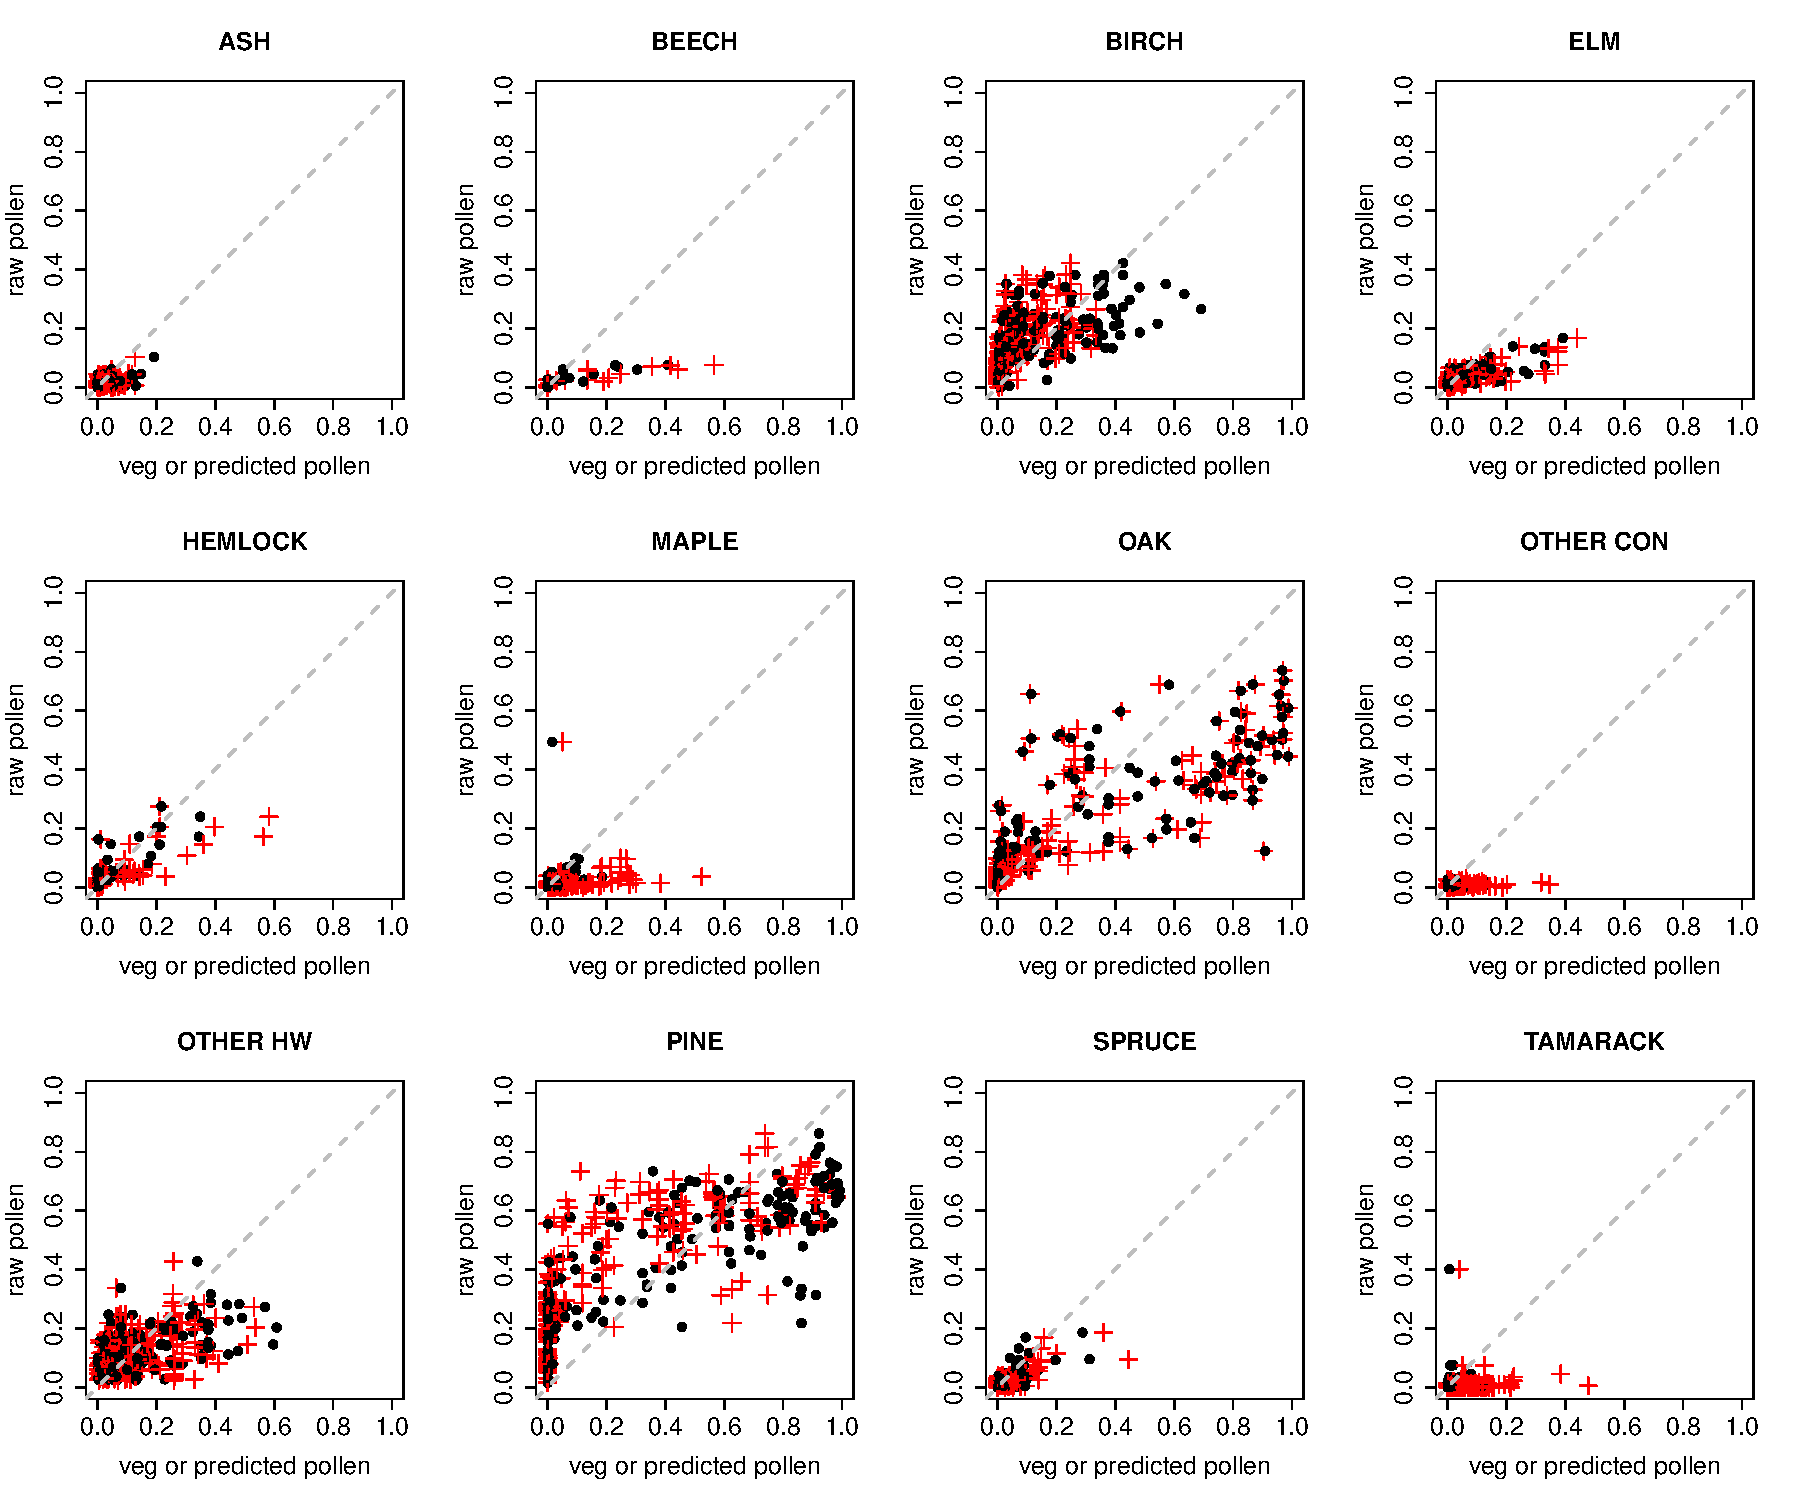
\includegraphics[width=7in]{figures/pollen_focal_scaled.pdf}
% \caption{}
% \label{fig:focal_scaled}
% \end{figure}

%PLS and pollen pie maps
\begin{figure}
\centering
\begin{tabular}{c}
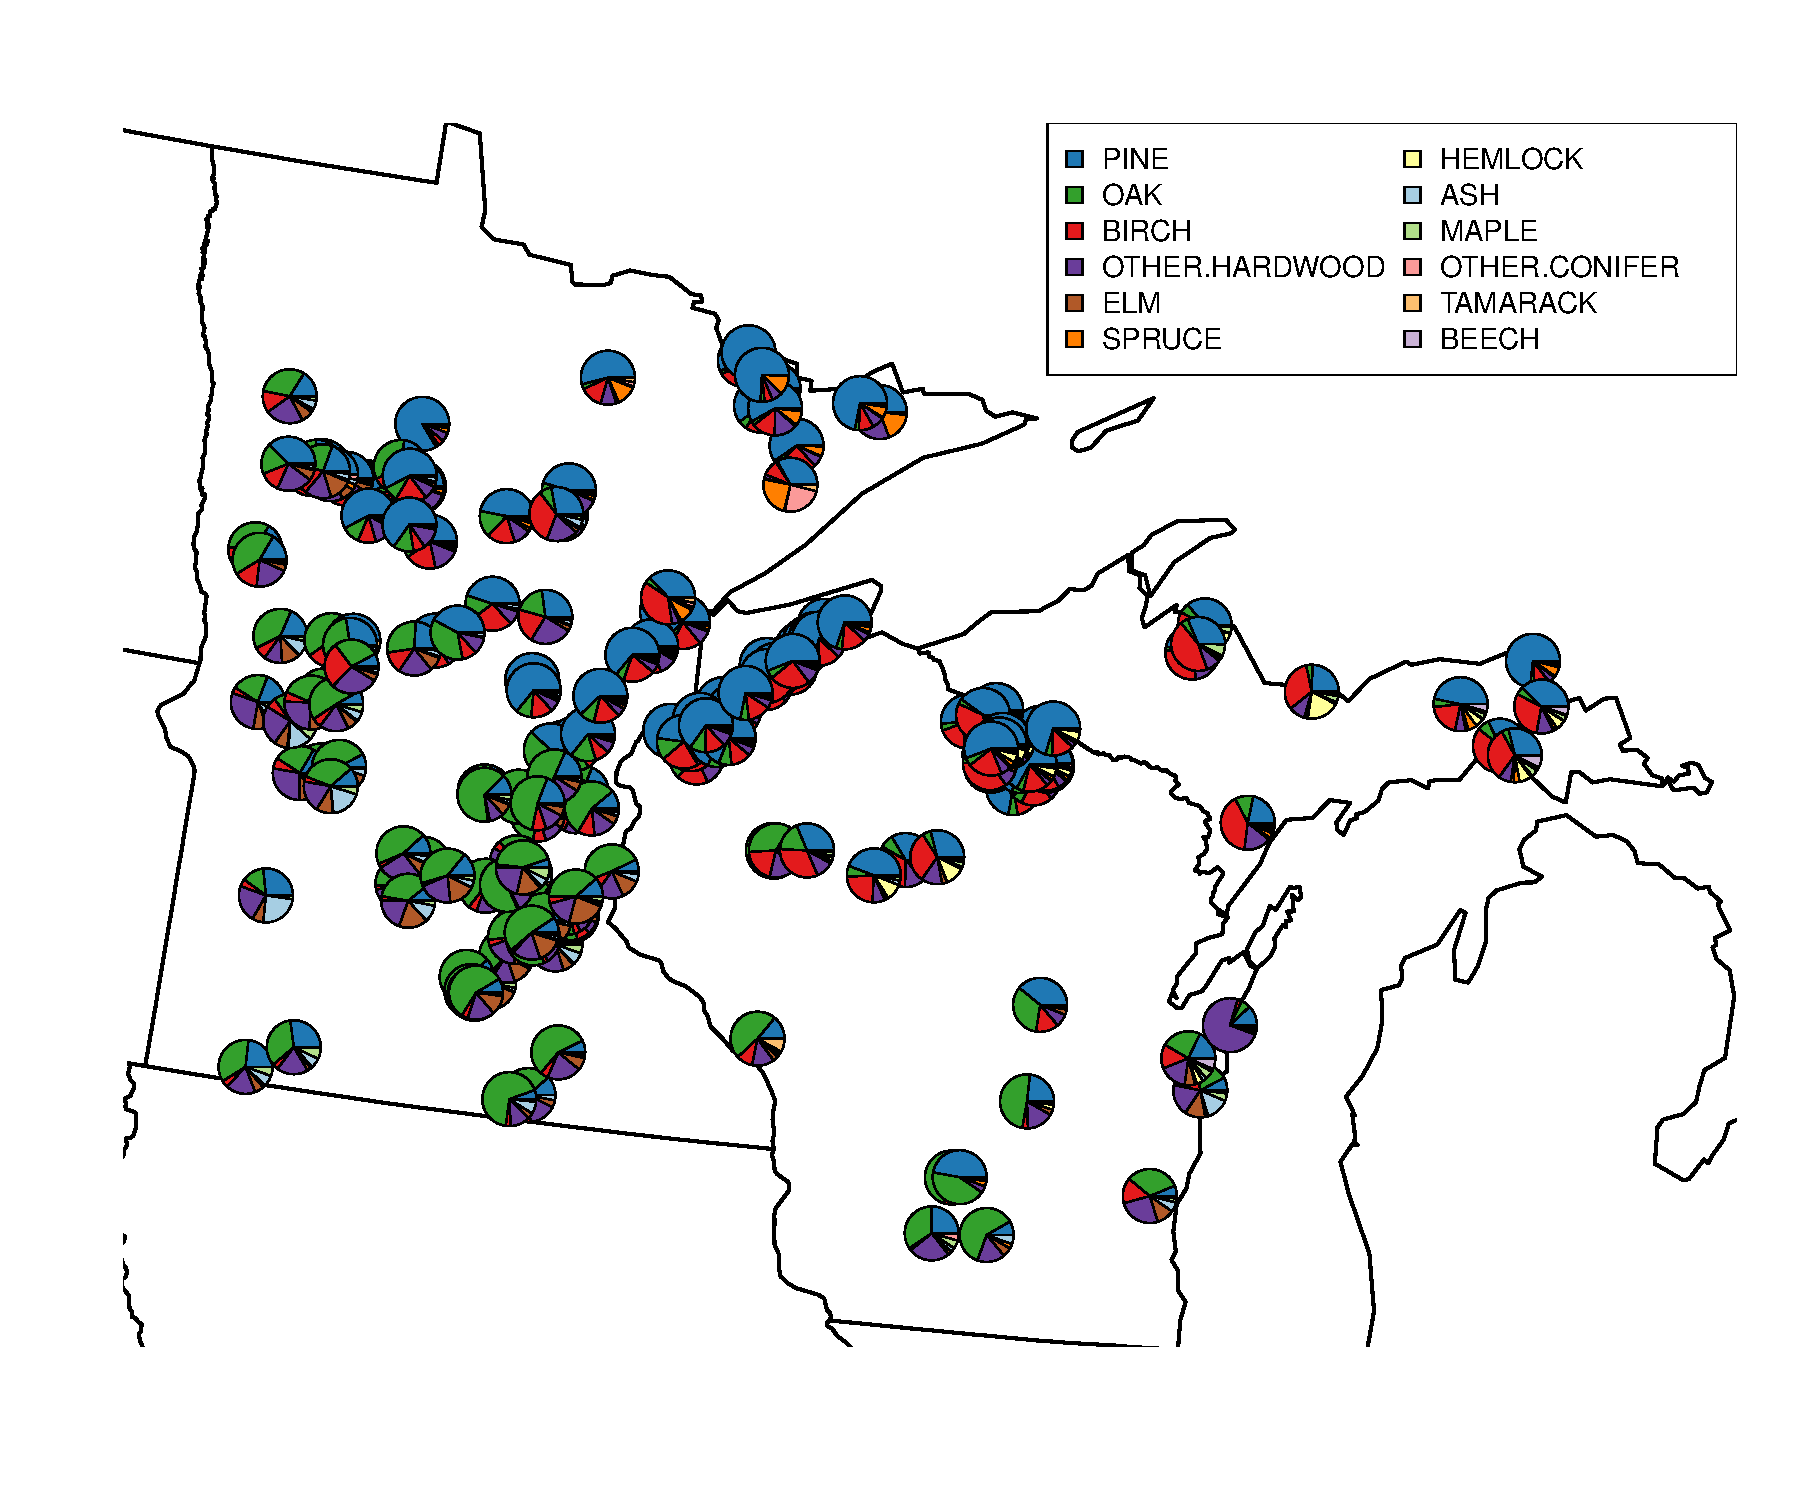
\includegraphics[width=5in]{figures/pie_plot_pollen_UMW_v01.pdf} \\
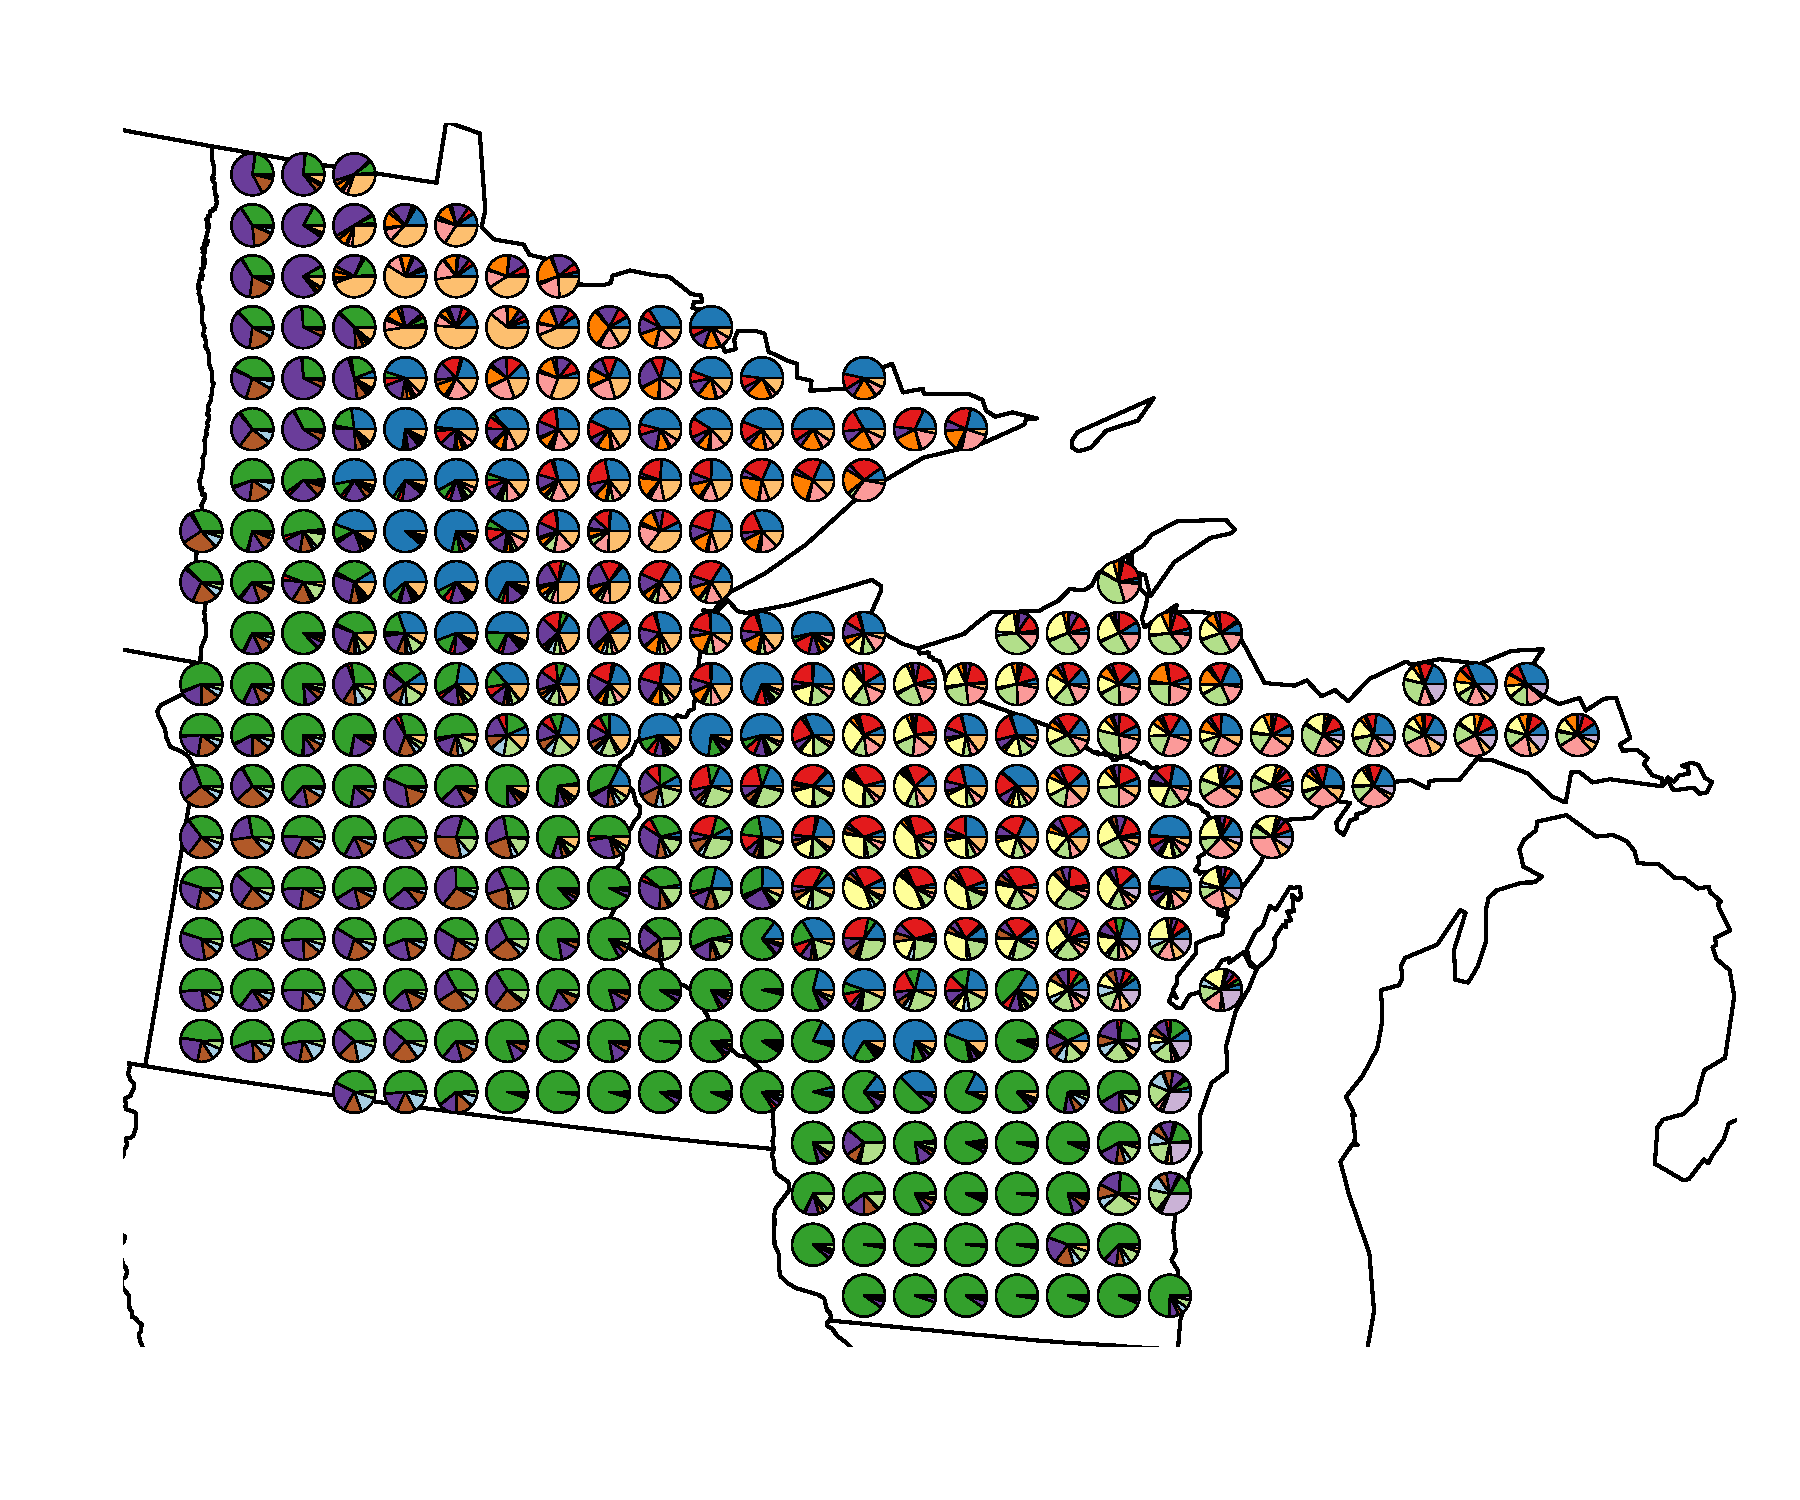
\includegraphics[width=5in]{figures/pie_plot_pls_UMW_v01.pdf}
\end{tabular}
\caption{Pie maps depicting the relative composition of pollen (top)
  and PLS vegetation (bottom) from the data. Note that the PLS data
  has been aggregated to a coarser resolution for illustrative
  purposes.}
\label{fig:pie}
\end{figure}

%veg and pollen heat maps: pine
\begin{figure}
\centering
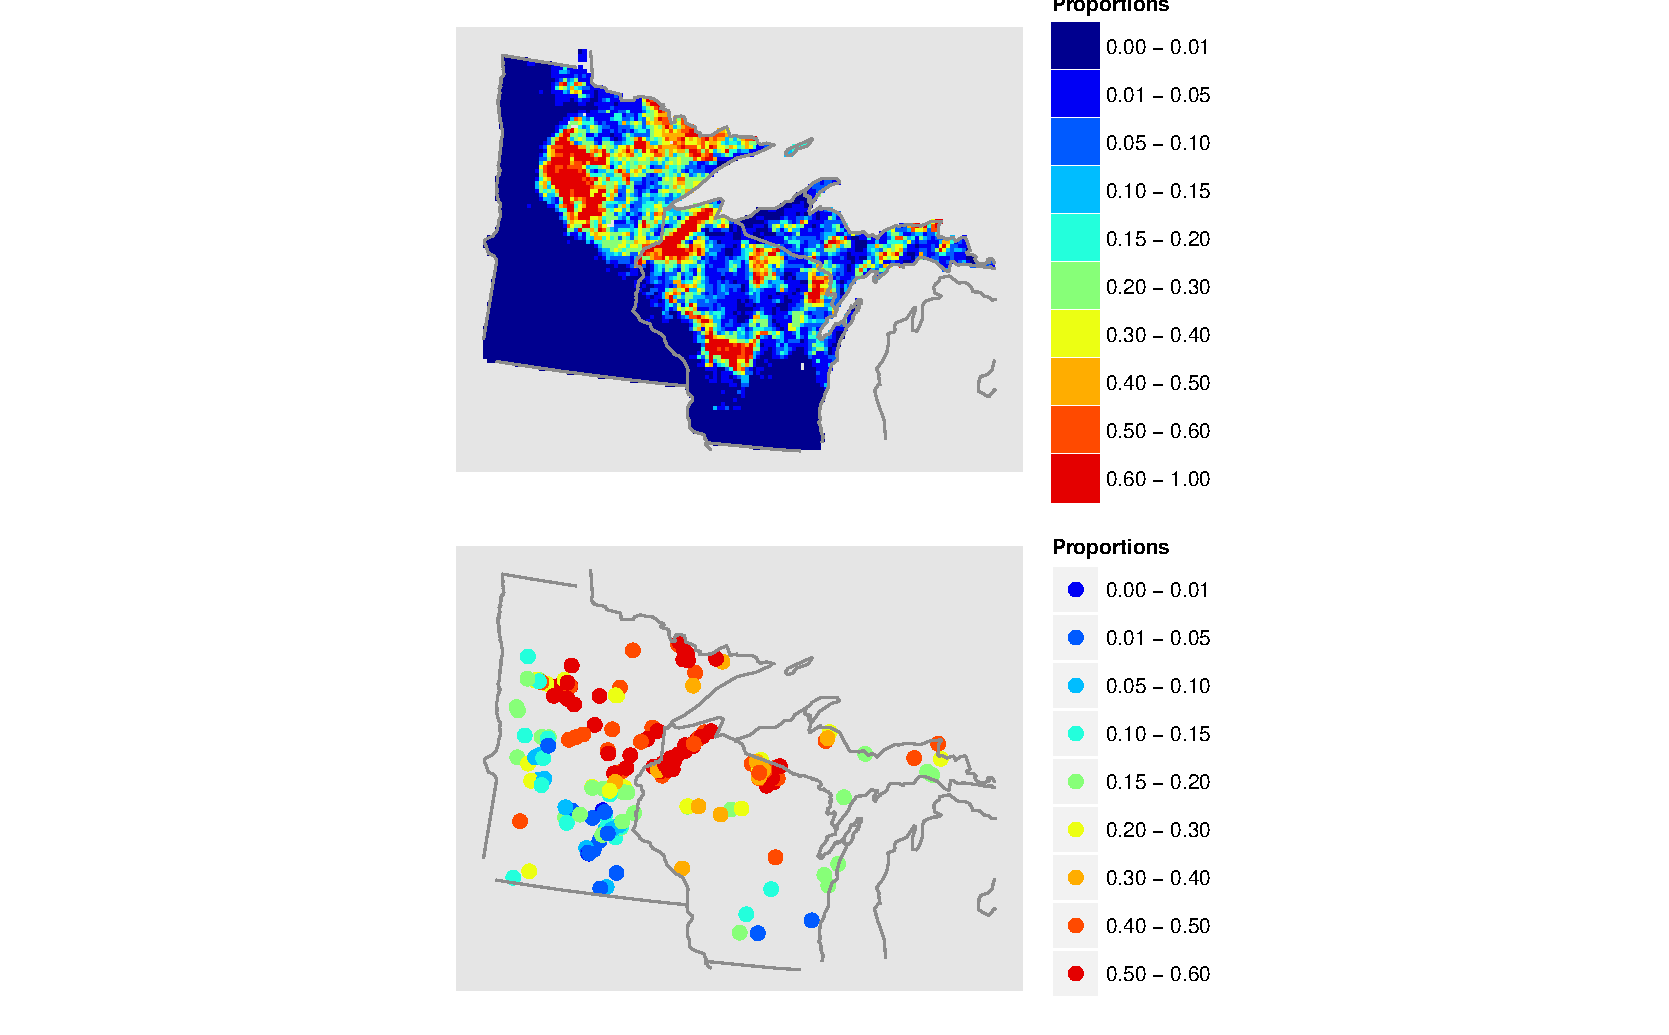
\includegraphics[width=7in]{figures/maps_compare_PINE.pdf}
\caption{Heat maps showing the range limits of Pine in the PLS composition data (top) and the sediment pollen (bottom).}
\label{fig:compare_maps_PINE}
\end{figure}

%veg and pollen heat maps: birch
\begin{figure}
\centering
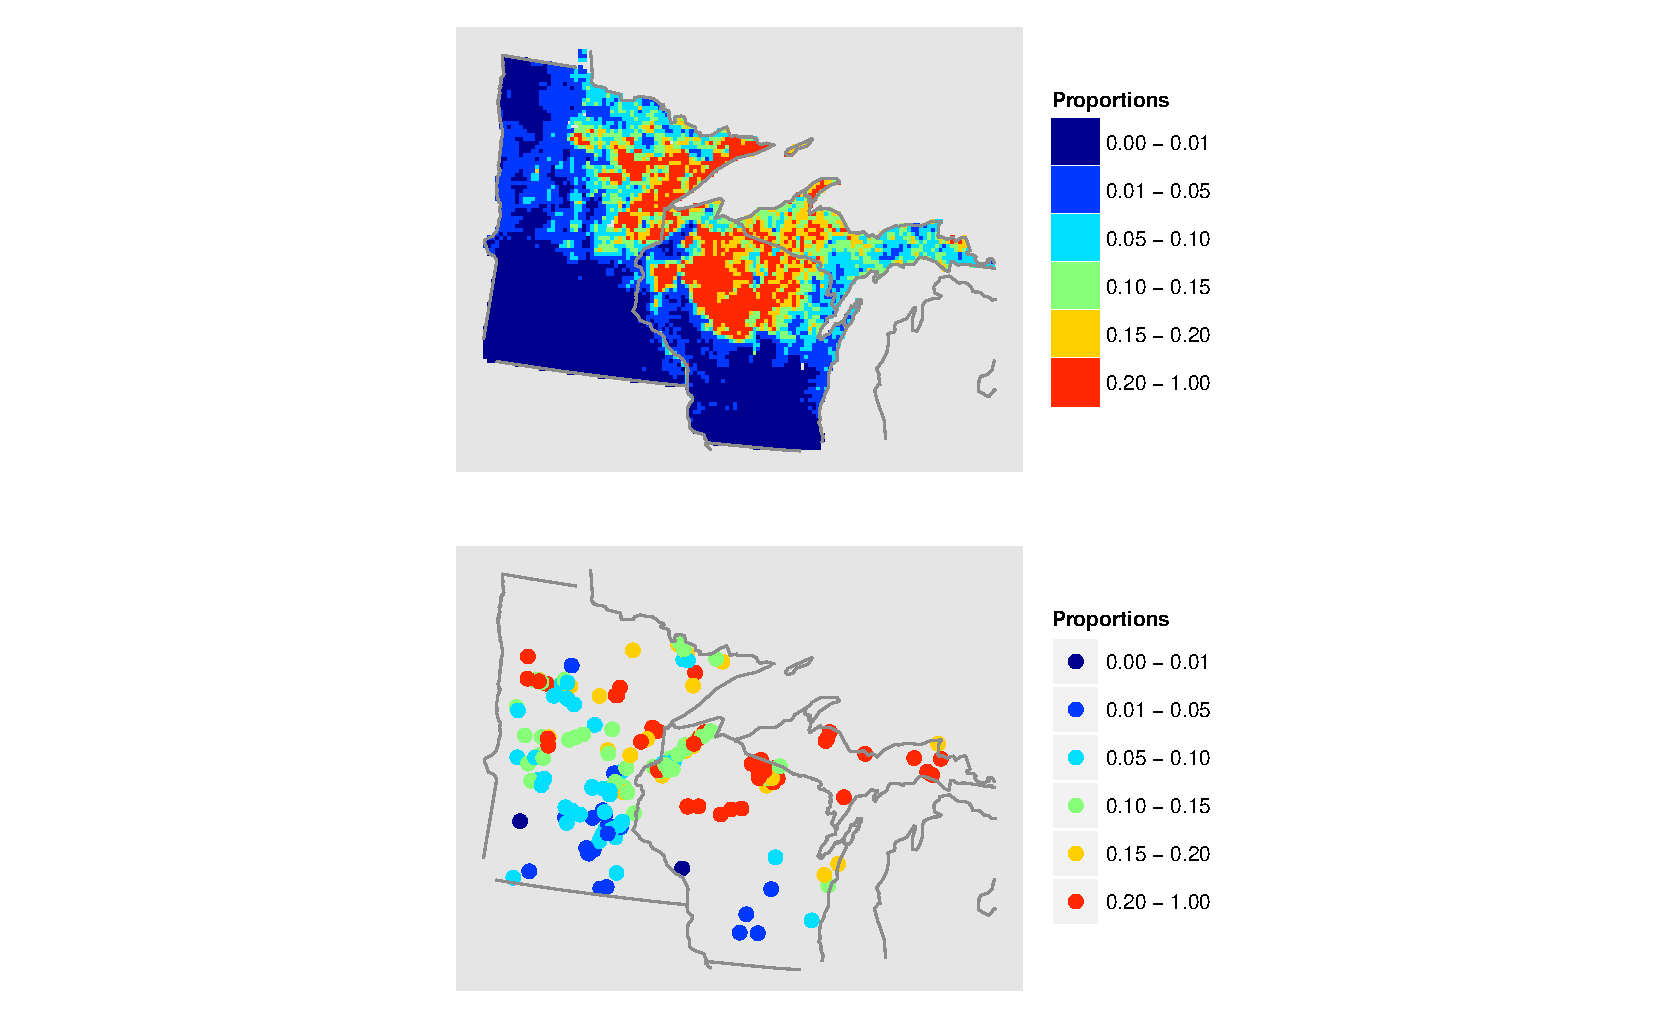
\includegraphics[width=7in]{figures/maps_compare_BIRCH.pdf}
\caption{Heat maps showing the range limits of Birch in the PLS composition data (top) and the sediment pollen (bottom)}
\label{fig:compare_maps_PINE}
\end{figure}

%pollen raw versus scaled focal
\begin{figure}
\centering
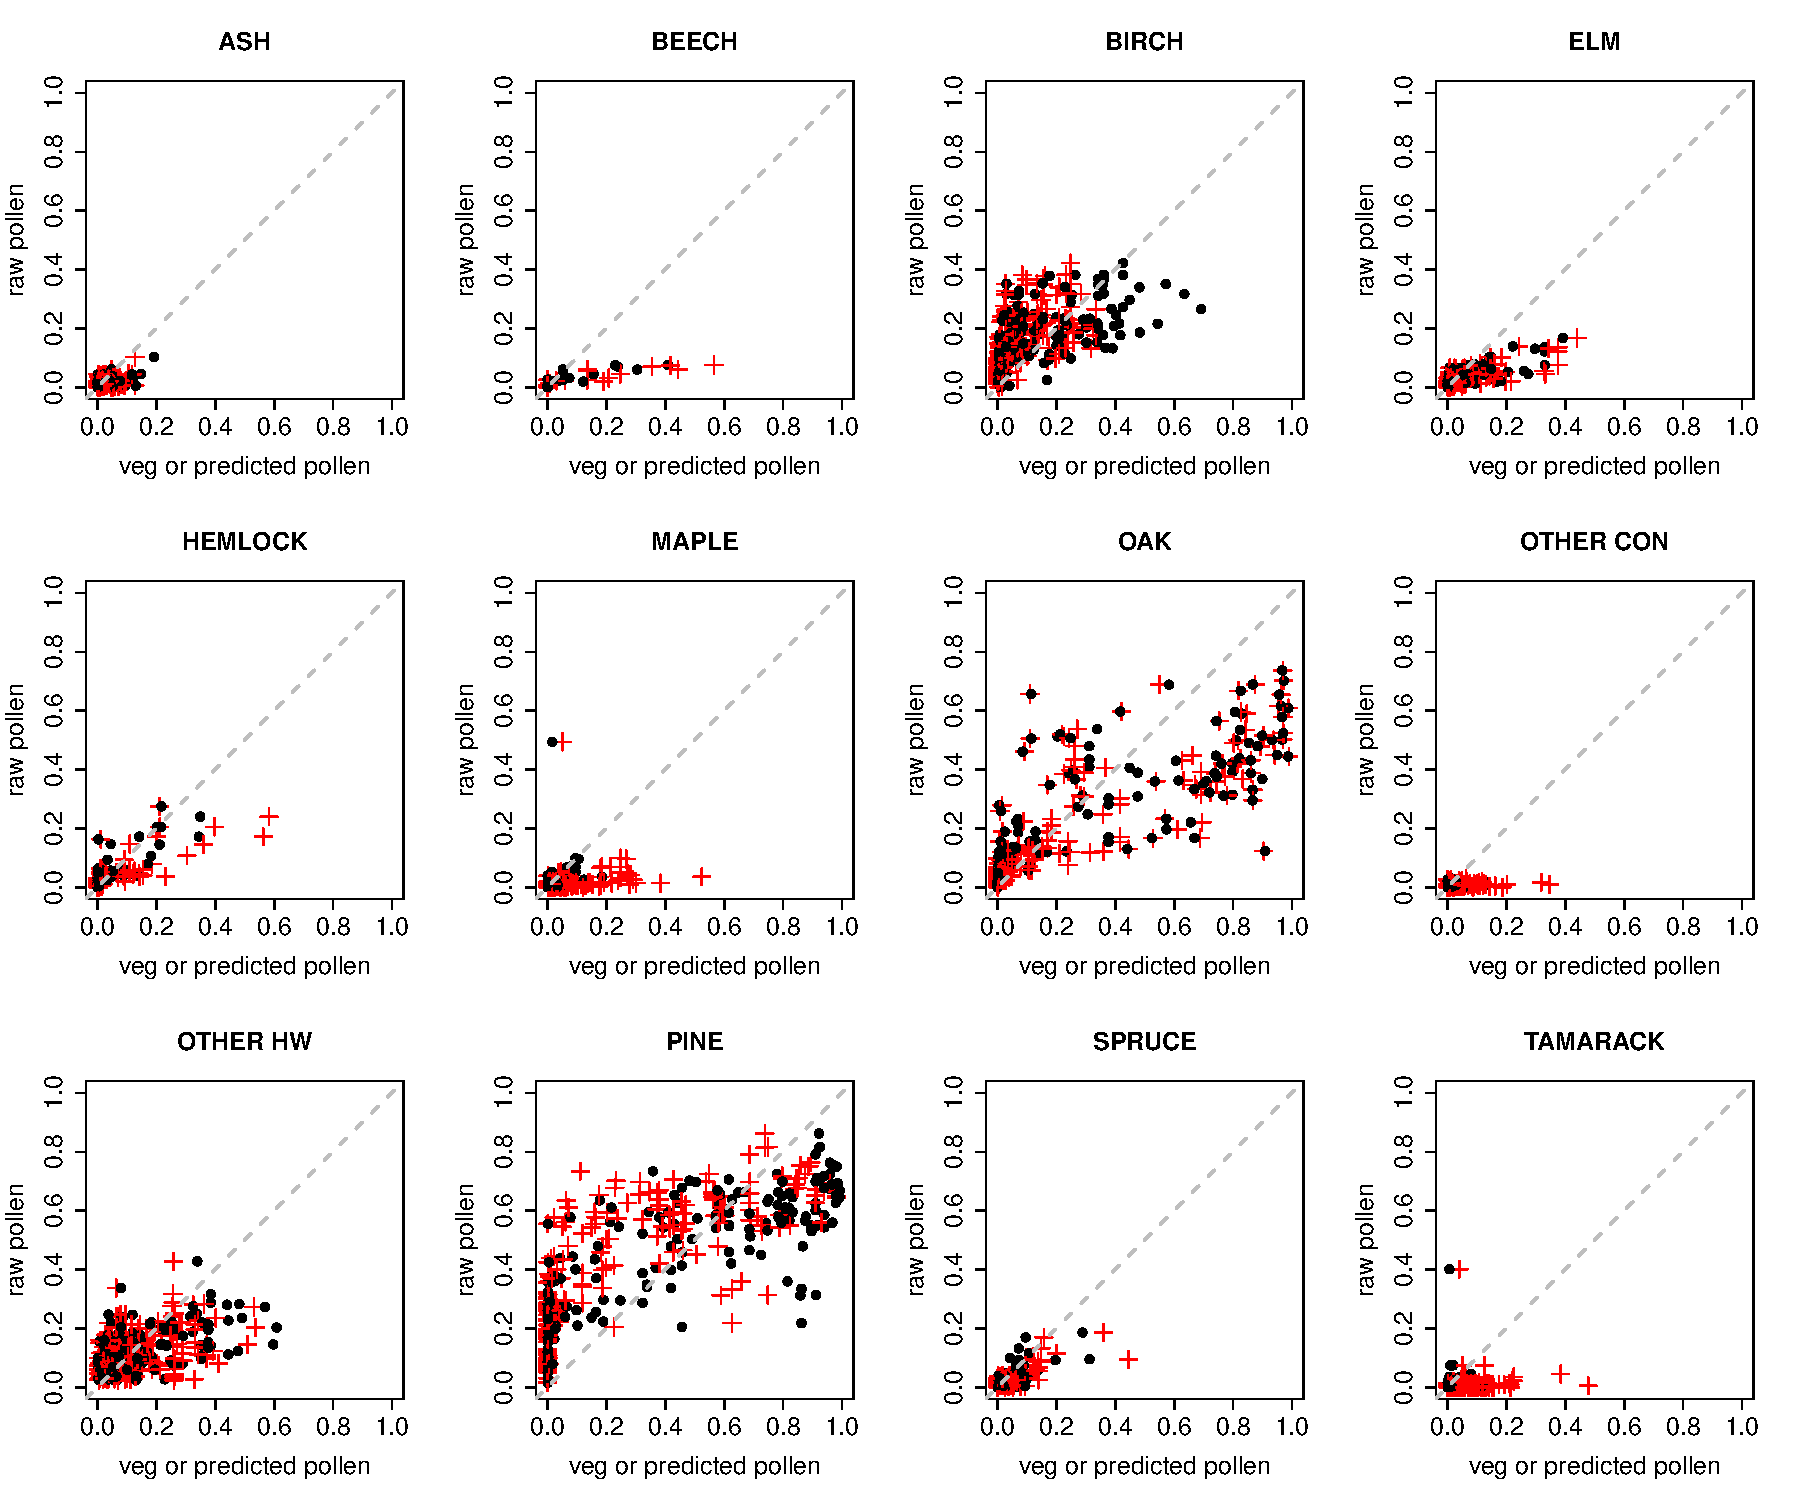
\includegraphics[width=7in]{figures/pollen_focal_scaled.pdf}
\caption{Pollen proportions plotted against local vegetation proportions (red crosses) or local vegetation proportion scaled by $\phi$ (black dots), by taxon.}
\label{fig:focal_scaled}
\end{figure}

%pollen raw versus predicted
\begin{figure}
\centering
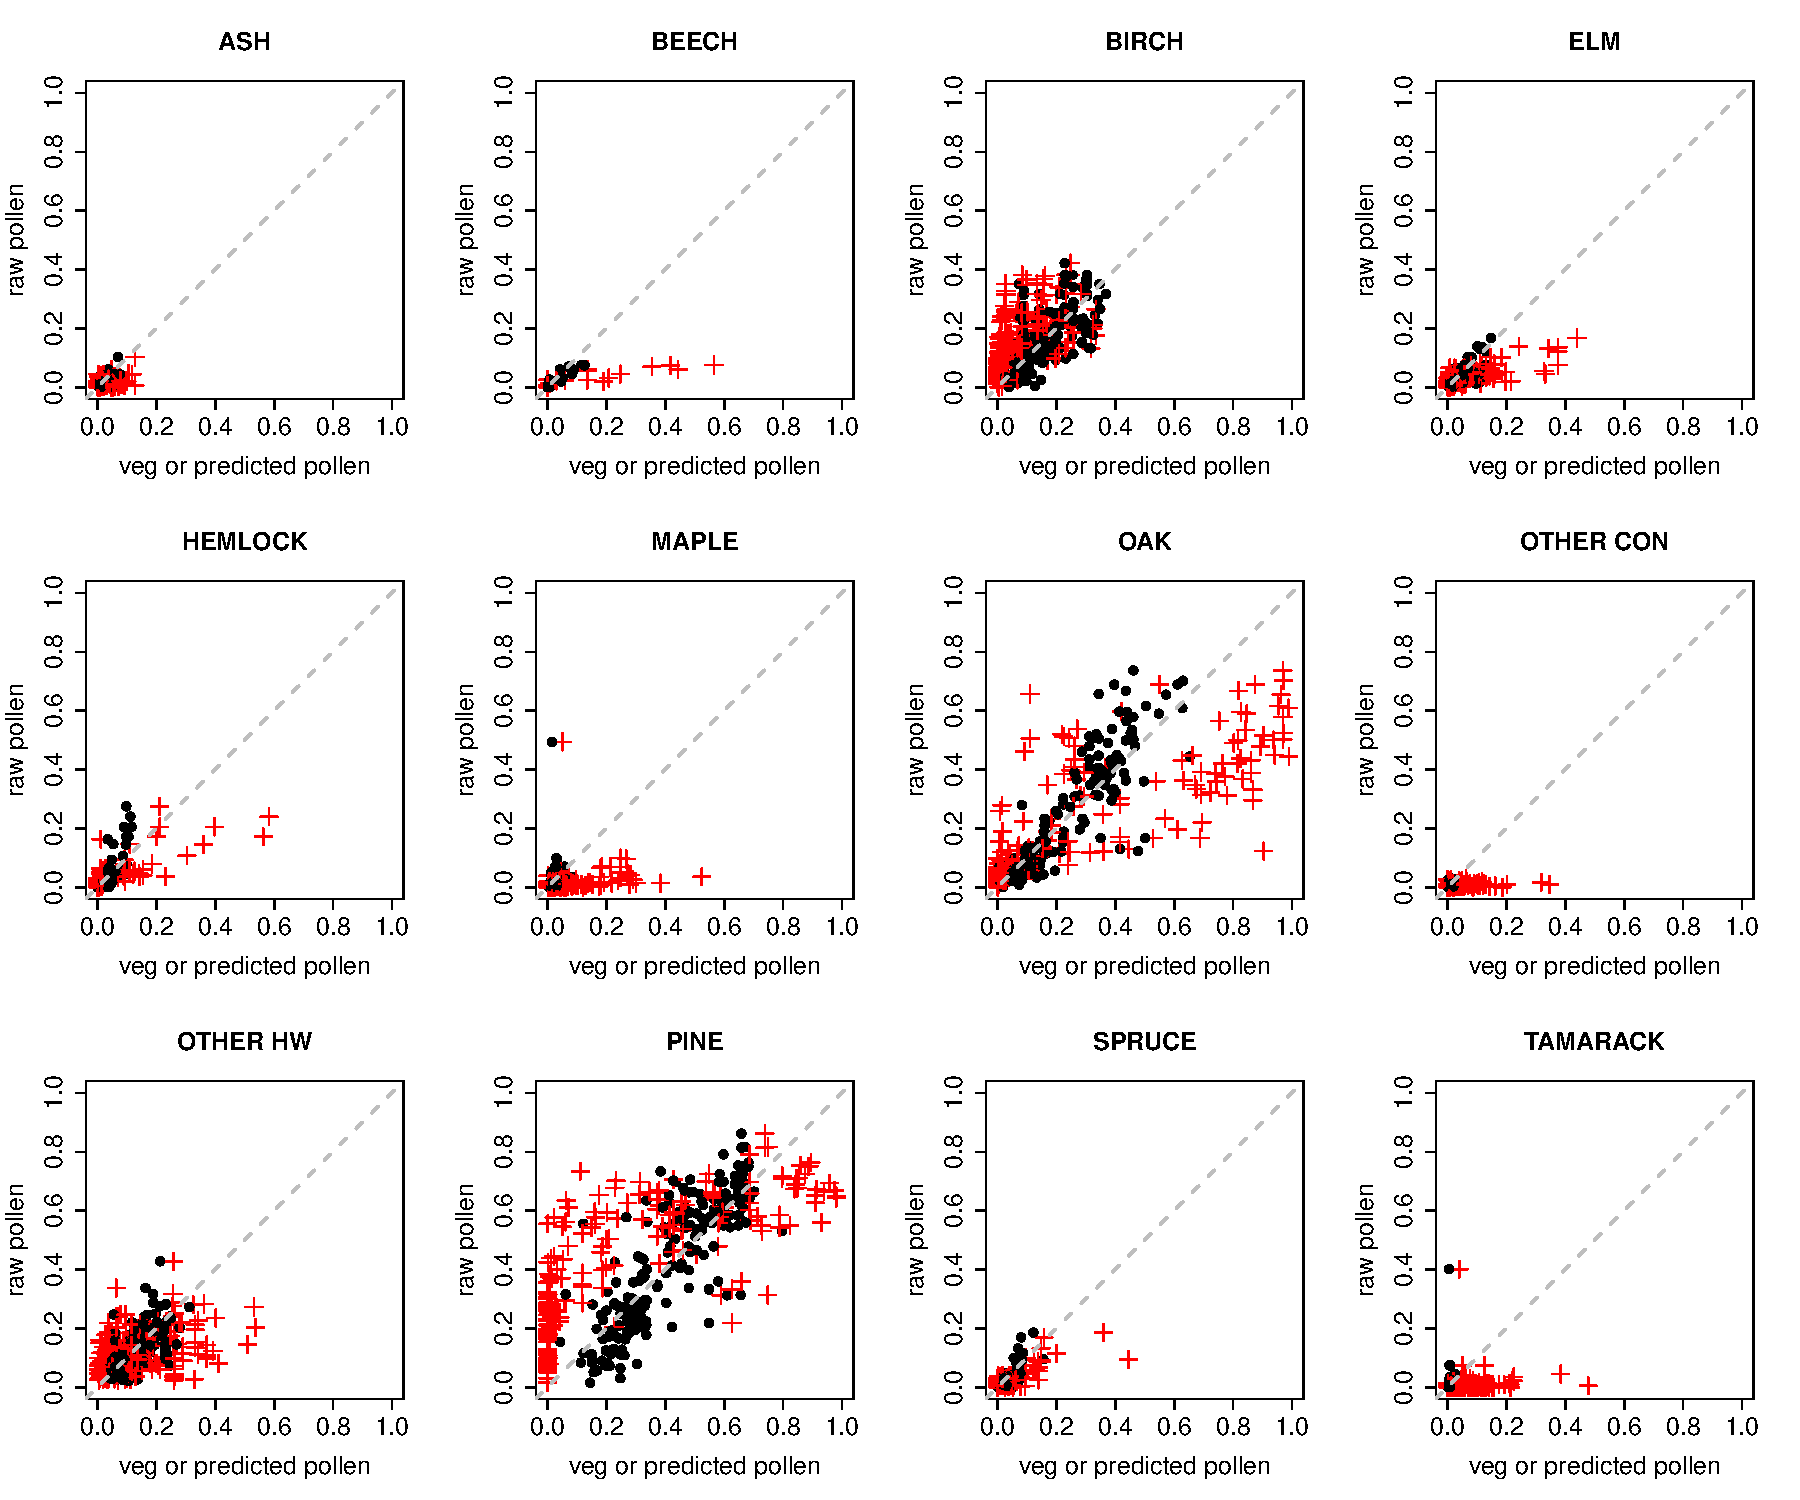
\includegraphics[width=7in]{figures/pollen_preds.pdf}
\caption{Pollen proportions plotted against local vegetation proportions (red crosses) or model-predicted pollen (black dots), by taxon.}
\label{fig:preds}
\end{figure}

%phi (differential production)
\begin{figure}
\centering
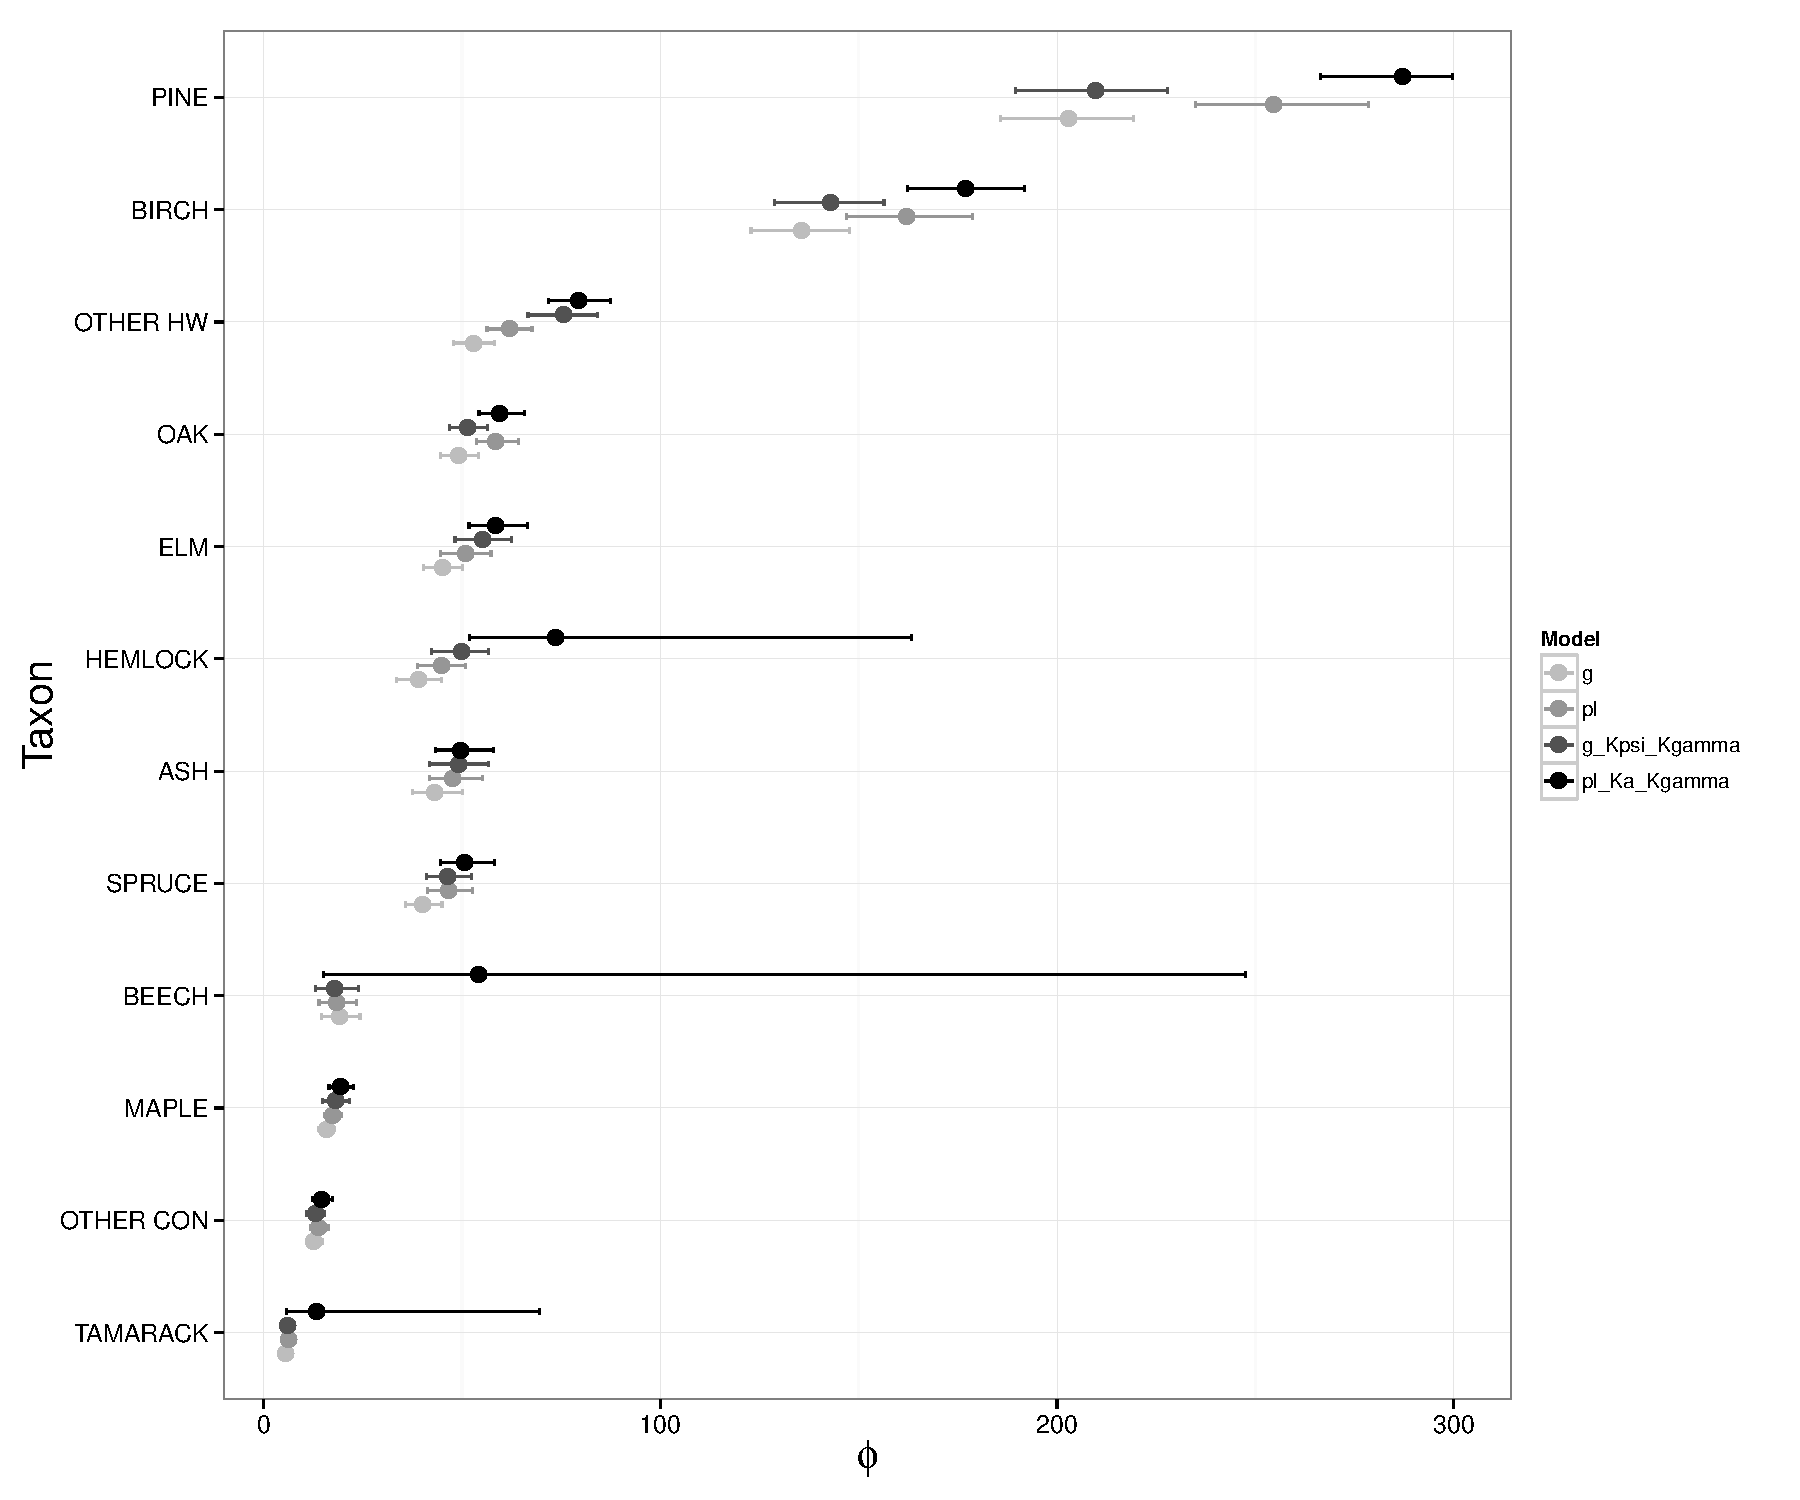
\includegraphics[width=7in]{figures/phi.pdf}
\caption{Mean values and 95\% credible intervals for the estimated values of the differential production parameter $\phi$.}
\label{fig:phi}
\end{figure}

%proportion pollen versus radius
\begin{figure}
\centering
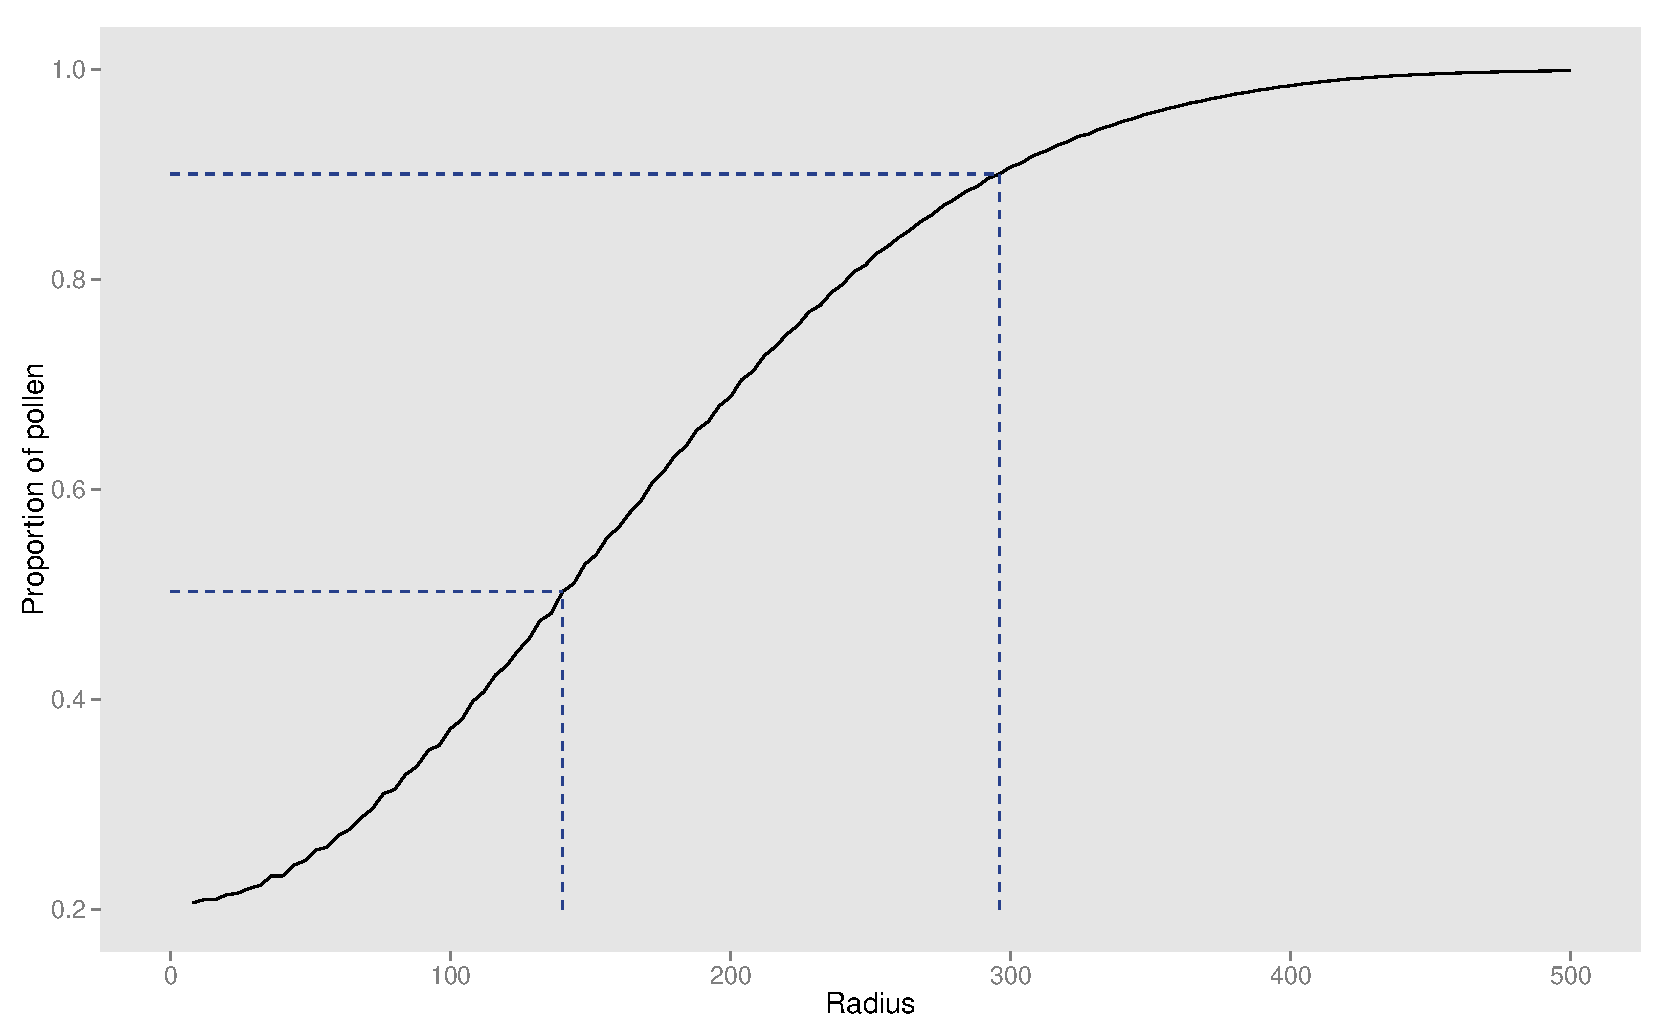
\includegraphics[width=7in]{figures/dispersal_vs_distance.pdf}
\caption{Here we consider pollen produced by a focal cell, and plot the proportion of deposited pollen as a function of the radius of a circle centered at the focal cell.}
\label{fig:dvd}
\end{figure}

%psi: vary psi case
\begin{figure}
\centering
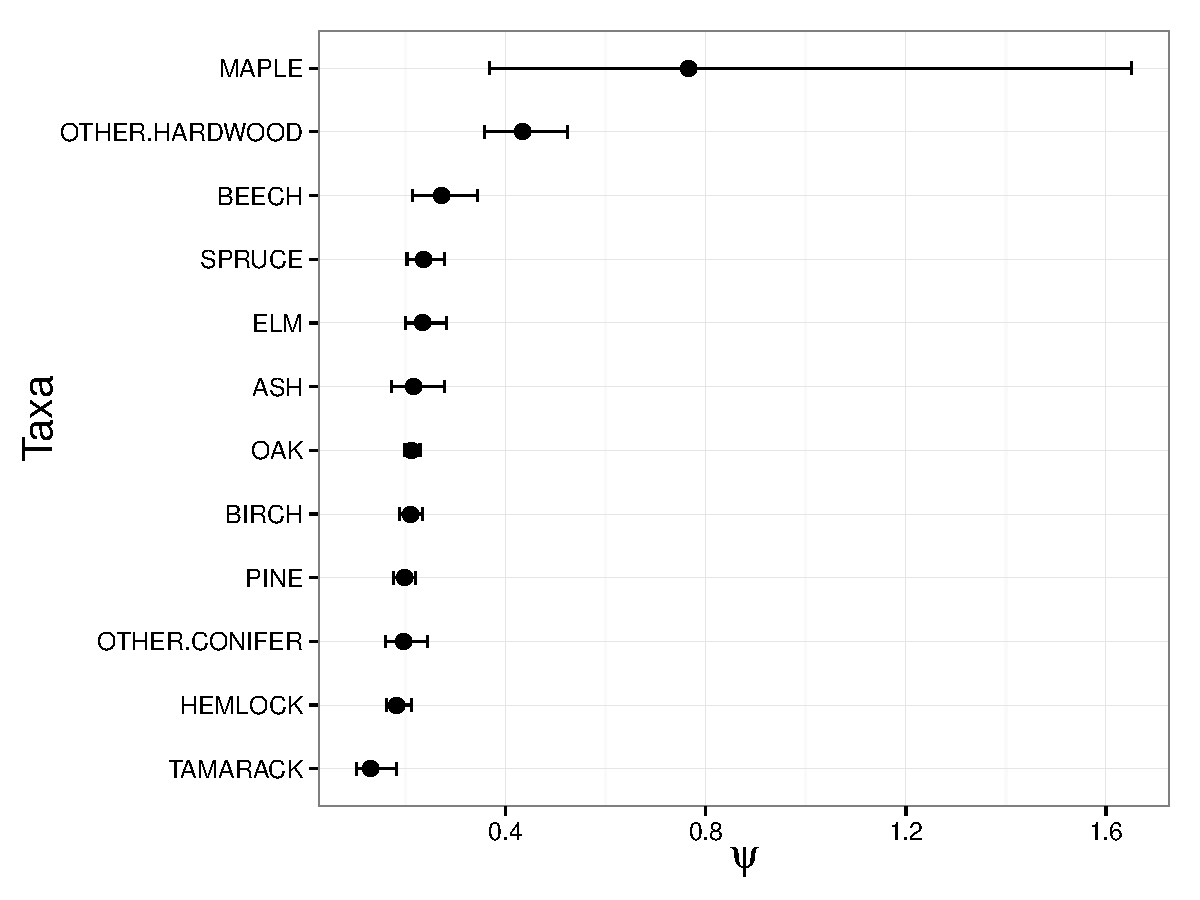
\includegraphics[width=7in]{figures/psi_vary_psi.pdf}
\caption{Mean values of 95\% credible intervals for the estimated values of the dispersal kernel spread $\psi$ for the case where we let $\psi$ vary by taxon.}
\label{fig:psi_vary_psi}
\end{figure}

%phi: vary phi case
\begin{figure}
\centering
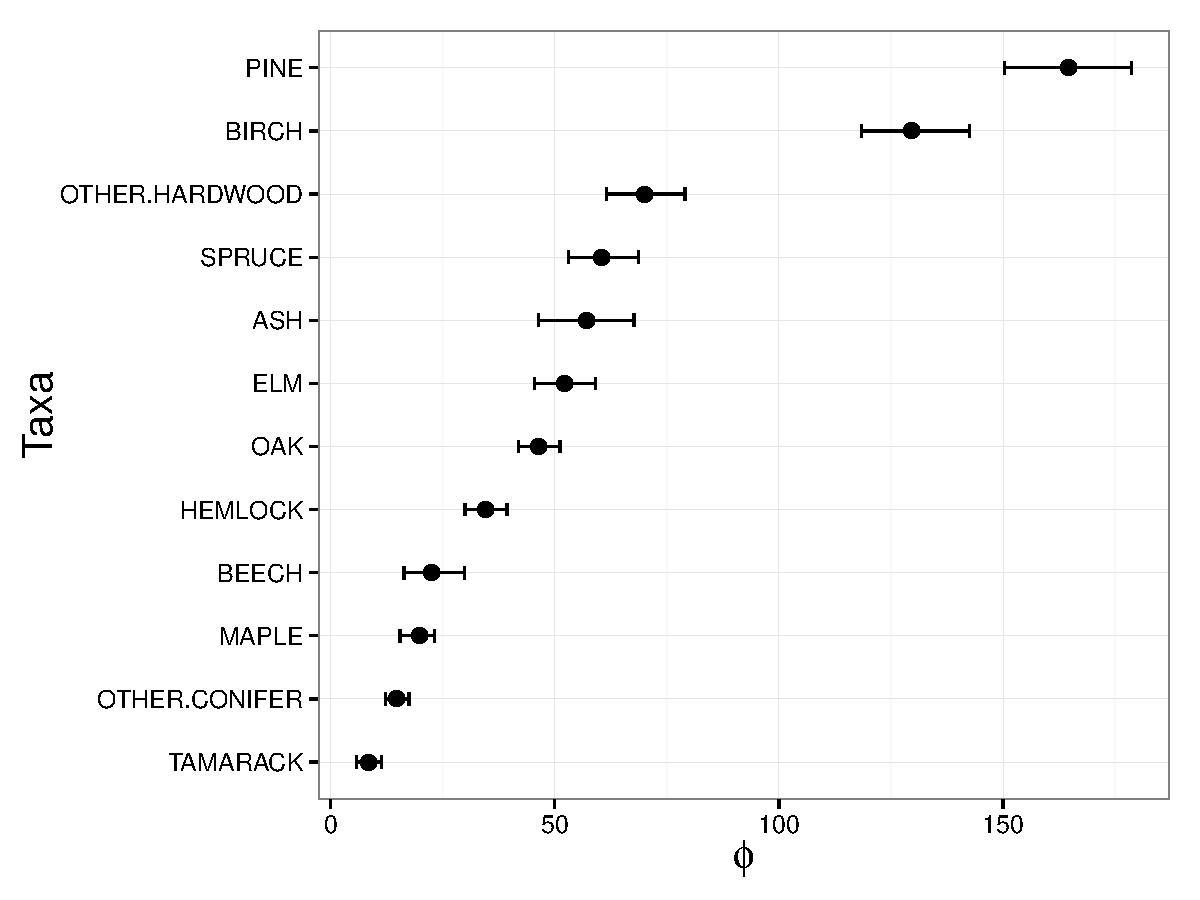
\includegraphics[width=7in]{figures/phi_vary_psi.pdf}
\caption{Mean values of 95\% credible intervals for the estimated values of the differential production parameter $\phi$ for the case where $\psi$ varied by taxon.}
\label{fig:phi_vary_psi}
\end{figure}

%potential pollen maps by taxon
\begin{figure}
\centering
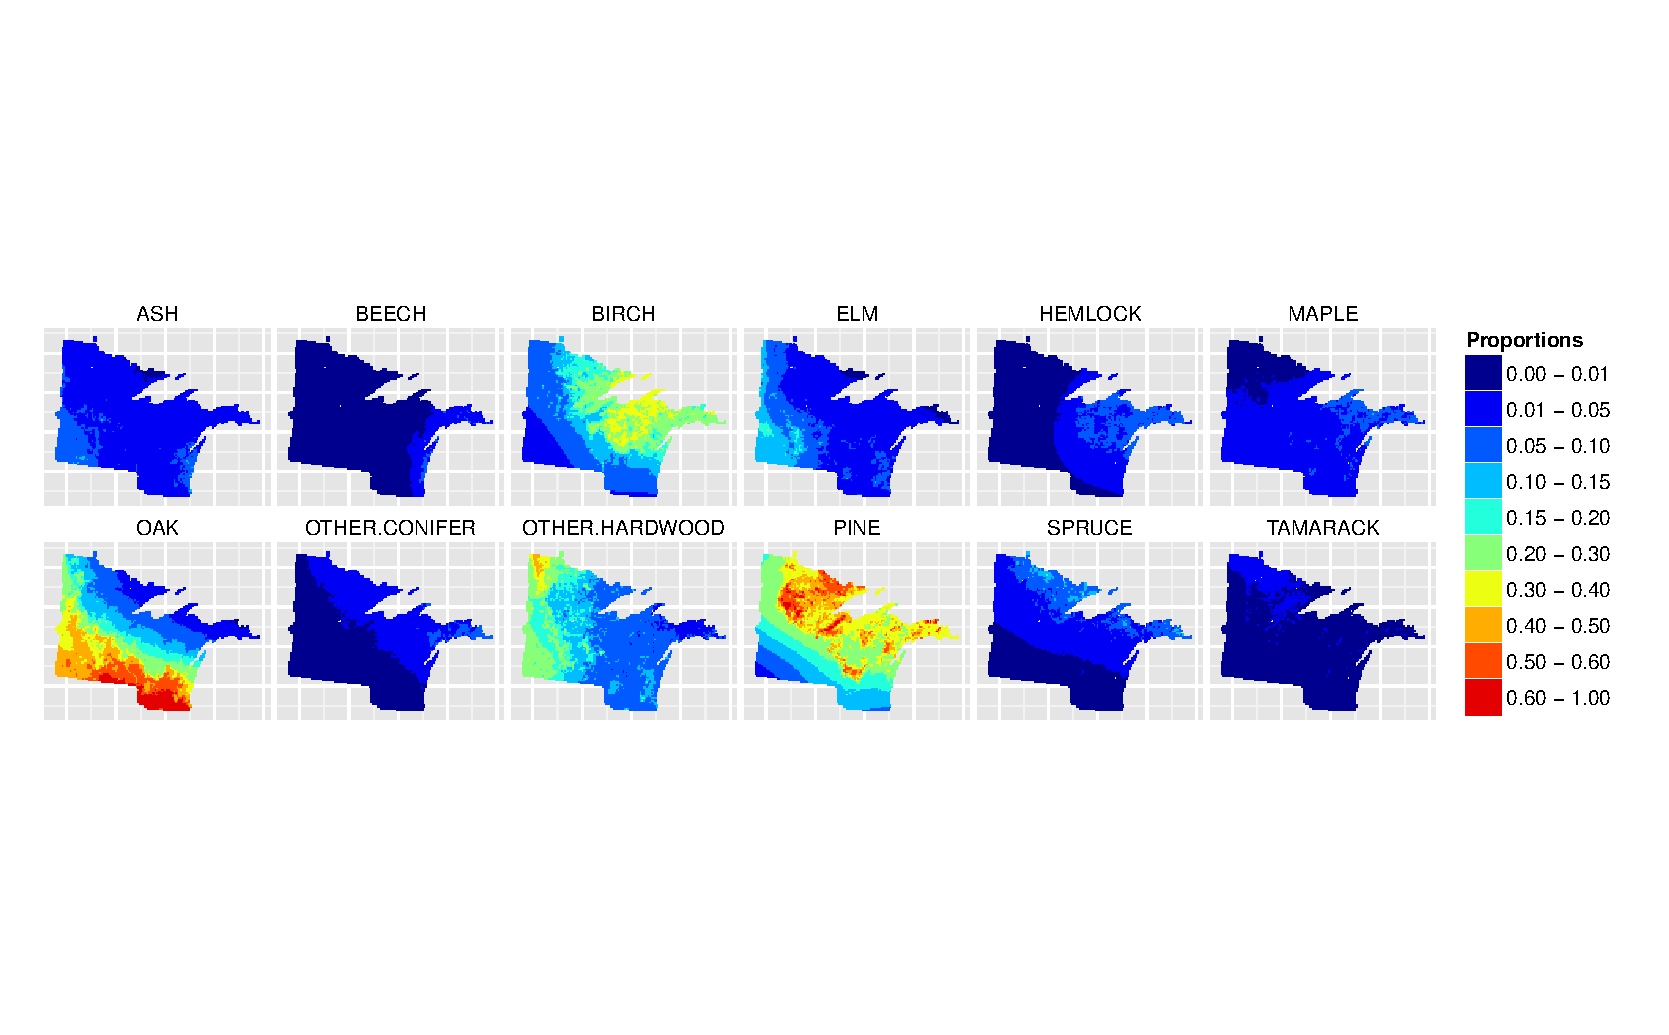
\includegraphics[width=7in]{figures/maps_pollen.pdf}
\caption{Heat maps of model-predicted pollen for each grid cell in the domain, by taxon.}
\label{fig:maps_pollen}
\end{figure}

%PLS data maps by taxon
\begin{figure}
\centering
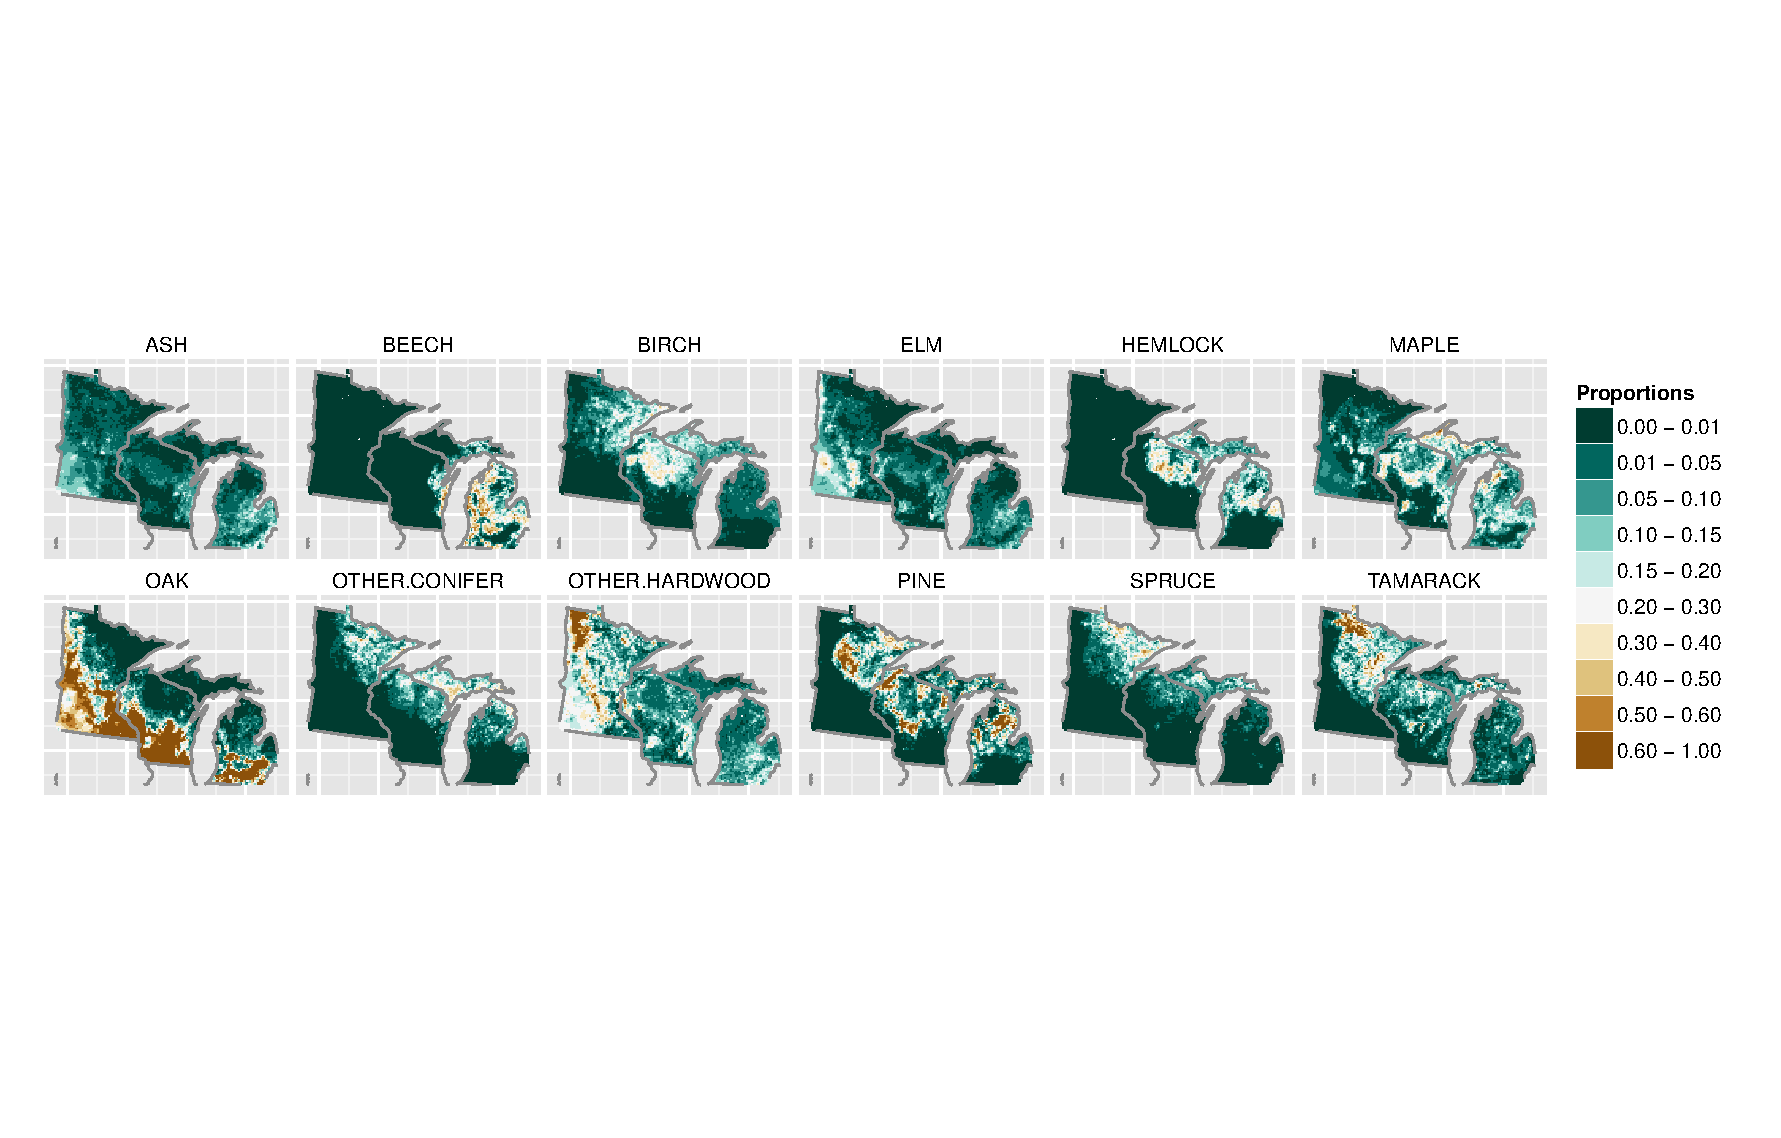
\includegraphics[width=7in]{figures/maps_veg.pdf}
\caption{Heat maps of the PLS data, by taxon.}
\label{fig:maps_pollen}
\end{figure}







\newpage
\vspace{2in}
\begin{appendices}
\section{}
\label{append}
\singlespacing
\begin{table}[H]
\begin{center}
\begin{tabular}{c*{2}{ r@{.}l @{ (} r@{.} l@{, } r@{.}l @{) \ \ }}}
\toprule
%                &   \multicolumn{2}{c}{Model} \\
% Common name    & $\gamma$ (Variable Gaussian) & $\gamma$ (Variable Power-law) \\  \midrule
%            Ash & 6.24e-2 (7.15e-3, 1.64e-1)   & 3.87e-2 (3.55e-4, 1.07e-1)    \\
%          Beech & 3.12e-1 (1.29e-1, 5.35e-1)   & 1.69e-1 (1.06e-2, 4.90e-1)    \\
%          Birch & 9.90e-2 (3.71e-2, 1.58e-1)   & 2.77e-2 (5.69e-4, 7.82e-2)    \\
%            Elm & 1.48e-1 (7.79e-2, 2.22e-1)   & 1.65e-1 (8.70e-2, 2.38e-1)    \\
%            Fir & 8.12e-2 (5.21e-3, 1.96e-1)   & 4.16e-2 (3.23e-4, 1.46e-1)    \\
%        Hemlock & 4.63e-1 (3.67e-1, 5.53e-1)   & 2.70e-1 (8.76e-2, 4.52e-1)    \\
%          Maple & 1.83e-1 (8.79e-2, 2.84e-1)   & 1.98e-1 (7.70e-2, 3.01e-1)    \\
%            Oak & 2.41e-1 (1.82e-1, 3.03e-1)   & 5.16e-2 (2.60e-3, 1.26e-1)    \\
% Other Hardwood & 4.73e-2 (3.07e-3, 8.67e-2)   & 5.32e-2 (1.58e-3, 1.05e-1)    \\
%           Pine & 2.49e-1 (2.14e-1, 2.82e-1)   & 2.11e-2 (3.12e-3, 4.86e-2)    \\
%         Spruce & 2.37e-1 (1.46e-1, 3.29e-1)   & 1.44e-1 (2.41e-2, 2.86e-1)    \\
%       Tamarack & 4.25e-1 (2.23e-1, 6.48e-1)   & 3.66e-1 (2.09e-2, 6.22e-1)    \\ \bottomrule
%               &   \multicolumn{2}{c}{Model} \\
Common name    & \multicolumn{6}{l}{$\gamma$ (Variable Gaussian)} & \multicolumn{6}{l}{$\gamma$ (Variable Power-law)} \\  \midrule
           Ash & 0&060  & 0&0065 & 0&15  & 0&028  & 0&000081 & 0&098    \\
         Beech & 0&30   & 0&11   & 0&52  & 0&15   & 0&0015   & 0&42    \\
         Birch & 0&088  & 0&032  & 0&15  & 0&015  & 0&000054 & 0&052    \\
           Elm & 0&13   & 0&070  & 0&20  & 0&13   & 0&051    & 0&19    \\
       Hemlock & 0&46   & 0&37   & 0&55  & 0&23   & 0&0091   & 0&44    \\
         Maple & 0&17   & 0&086  & 0&28  & 0&14   & 0&0023   & 0&26    \\
           Oak & 0&25   & 0&18   & 0&32  & 0&042  & 0&00017  & 0&12    \\
Other conifer  & 0&084  & 0&0076 & 0&21  & 0&037  & 0&000084 & 0&14    \\
Other hardwood & 0&041  & 0&0088 & 0&080 & 0&031  & 0&00058  & 0&071    \\
          Pine & 0&24   & 0&21   & 0&28  & 0&016  & 0&000073 & 0&049    \\
        Spruce & 0&25   & 0&16   & 0&33  & 0&15   & 0&014    & 0&26    \\
      Tamarack & 0&43   & 0&22   & 0&64  & 0&37   & 0&10     & 0&61    \\ \bottomrule
\end{tabular}
\caption{Estimates of parameter $\gamma$, indicating the proportion of
  locally sourced pollen for the variable Gaussian model in which
  $\psi$ and $\gamma$ both vary by taxon and the variable Power-law
  kernel model in which $a$ and $\gamma$ vary by taxon. For the base
  models, $\gamma$ was estimated to be $0.21 (0.19, 0.23) $ for the
  Gaussian kernel model and $0.046 (0.013, 0.078) $ for the Power-law
  kernel model.}
\end{center}
\label{table:gamma}
%\vspace{2cm}
\end{table}

\newpage
\begin{table}[H]
\begin{center}
\begin{tabular}{ccc} 
\toprule
               &   \multicolumn{2}{c}{Model} \\
               & Variable Gaussian           & Variable Power-law \\  \midrule
Common name    & $\psi$             & $a$         \\  \midrule
           Ash & 0.29 (0.22, 0.39)  & 0.079 (0.033, 0.25)    \\
         Beech & 0.25 (0.20, 0.34)  & 0.0027 (0.00045, 0.018)    \\
         Birch & 0.16 (0.14, 0.18)  & 0.014 (0.0082, 0.026)    \\
           Elm & 0.36 (0.27, 0.49)  & 0.20 (0.067, 0.81)    \\
           Fir & 0.22 (0.19, 0.26)  & 0.0042 (0.0010, 0.017)    \\
       Hemlock & 0.26 (0.16, 0.44)  & 0.047 (0.0034, 0.33)    \\
         Maple & 0.22 (0.19, 0.24)  & 0.015 (0.0078, 0.027)    \\
           Oak & 0.19 (0.14, 0.24)  & 0.019 (0.0043, 0.055)    \\
Other Hardwood & 0.36 (0.31, 0.43)  & 0.18 (0.095, 0.32)    \\
          Pine & 0.15 (0.14, 0.17)  & 0.0052 (0.0037, 0.0080)    \\
        Spruce & 0.26 (0.22, 0.31)  & 0.036 (0.014, 0.10)    \\
      Tamarack & 0.23 (0.13, 0.55)  & 0.022 (0.00040, 0.50)    \\ \bottomrule
\end{tabular}
\end{center}
\end{table}


% For the base Gaussian kernel case, the spread parameter $\psi$ was
% estimated to be $204\,(192, 215)$ km. In the variable Gaussian model
% $\psi$ estimates ranged from 152 for pine to 361 for Other
% hardwood. For many taxa, 95\% credible intervals are large; this is
% especially true for Tamarack ($\psi$ of $230\,(128, 553)$. For the
% base Power-law model, the kernel parameters $a$ and $b$ were estimated
% to be $0.01\,(0.00829, 0.02)$ and $2.03\,(2.00, 2.12)$. For the
% variable Power-law model, the estimated $b$ value was almost identical
% to the base model $2.06\,(2.00, 2.16)$. The $a$ estimates ranged from
% $0.00268$ for beech to $0.203$ for elm.


% \pgfplotstableset{
% }


 % \begin{table}[h!]
 %  \begin{center}
 %    \caption{XXX.}
 %    \label{table1}



    \pgfplotstabletypeset[
      begin table=\begin{landscape}\begin{longtable},
      end table=\caption{A full list of sediment pollen sites in the %
                    Upper Midwestern USA considered for inclusion in %
                    the calibration data set. Meta data provided %
                    includes site name (Site), Neotoma or given %
                    identification number (ID), latitude (Lat) and %
                    longitude (Long), principal investigator (PI), %
                    depth of the settlement-era pollen sample (Depth; %
                    may be recorded as either depth from upper most %
                    sediment layer, or from lake surface), an %
                    indication if the dataset came from Neotoma %
                    (Neotoma), an indication as to whether the dataset %
                    is included in the final calibration data set %
                    (Calibration), and in the case a site is not %
                    included (Calibration value of N), then a note %
                    indication the reason for inadmissibility %
                    (Notes). The reasons for inadmissibility are: A) %
                    Three or four experts did not assign a %
                    pre-settlement sample; B) Two experts did not %
                    assign a pre-settlement sample, and the two %
                    assigned pre-settlement samples were at least 300 %
                    years away from 1850 according to the default %
                    age-depth models; C) No core top.} %
                    \label{table:site-data}\end{longtable}\end{landscape},
      multicolumn names,
      col sep=comma,
      font=\small,
      display columns/0/.style={string type},
      display columns/1/.style={string type},
      display columns/4/.style={string type},
      display columns/6/.style={string type},
      display columns/7/.style={string type},
      display columns/8/.style={string type},
      empty cells with=\ ,
      every head row/.style={
		before row={\toprule},
		after row={\midrule\endhead}},
      every last row/.style={after row={\bottomrule\\}},
    ]{../../stepps-data/data/meta_v3.csv}



\include{figures_appendix}
\end{appendices}

\end{document}
